\documentclass[report]{jlreq}
\usepackage{global}
\usepackage{./local}
\subfiletrue
\def\assetspath{../}
\begin{document}


% ============================================================
%
% ============================================================
\chapter{基本群と被覆空間}

基本群と被覆空間について述べる。

% ----------------------------------------------------------------------------
%
% ----------------------------------------------------------------------------
\section{空間対}

空間対の概念を導入する。

\begin{definition}[空間対]
    \idxsym{category of pairs of spaces}{$\CatTopPair$}{空間対の圏}
    圏$\CatTopPair$を次のように定める:
    \begin{itemize}
        \item $\Ob(\CatTopPair)$は
            位相空間$X$とその部分空間$A \subset X$の対$(X, A)$の全体
        \item 各$(X, A), (Y, B) \in \Ob(\CatTopPair)$に対し、
            $\Ar((X, A), (Y, B))$は
            連続写像$f \colon X \to Y$であって$f(A) \subset B$なるものの全体
    \end{itemize}
    $\CatTopPair$を
    \term{空間対の圏}[category of pairs of spaces]{空間対の圏}[くうかんついのけん]
    という。
\end{definition}

\begin{definition}[空間対のホモトピー]
    $f, g \colon (X, A) \to (Y, B)$を空間対の射とする。
    $f, g$が\term{ホモトピック}[homotopic]{ホモトピック!空間対---}[ほもとぴっく]
    であるとは、
    空間対の射$H \colon (X \times I, A \times I) \to (Y, B)$であって
    $H \colon X \times I \to Y$が
    $f \colon X \to Y$を$g \colon X \to Y$に
    つなぐホモトピーであるようなものが存在することをいう。
    空間対の
    \term{ホモトピー同値}[homotopy equivalent]{ホモトピー同値!空間対---}[ほもとぴーどうち]
    や
    \term{ホモトピー同値射}[homotopy equivalence]{ホモトピー同値射!空間対---}[ほもとぴーどうちしゃ]
    も同様に定義する。
\end{definition}

% ------------------------------------------------------------
%
% ------------------------------------------------------------
\section{ホモトピー}

ホモトピーについて述べる。
ホモトピーの概念は基本群やホモロジーの重要な基盤となる。

\subsection{ホモトピーの定義と基本性質}

\TODO{最初から空間対で定義する?}

\TODO{相対ホモトピーは後で導入すべき?
    空間対は包含だけど相対ホモトピーは固定だから違うもの?}

ホモトピーとは、大まかには2つの写像の間の連続的な変形を表すものである。

\begin{definition}[相対ホモトピー]
    \idxsym{homotopic maps rel $A$}{$f \simeq g \; \rel \; A$}{rel $A$ でホモトピックな写像}
    $f, g \colon X \to Y$を連続写像、
    $A \subset X$、
    $f = g \; \text{on} \; A$とする。
    連続写像$H \colon X \times I \to Y$であって
    \begin{alignat}{1}
        H(x, 0) &= f(x) \quad (\forall x \in X) \\
        H(x, 1) &= g(x) \quad (\forall x \in X) \\
        H(a, t) &= f(a) = g(a) \quad (\forall a \in A, \; t \in I)
    \end{alignat}
    をみたすものが存在するとき
    $f \simeqhe g \; \rel \; A$と書き、
    $f$と$g$は
    \term{rel $A$ でホモトピック}[homotopic rel $A$]{ホモトピック!相対---}
    であるという。
    $H$を$f$と$g$をつなぐ rel $A$な
    \term{相対ホモトピー}[relative homotopy]{ホモトピー!相対---}
    という。
\end{definition}

\begin{definition}[自由ホモトピー]
    \idxsym{homotopic maps}{$f \simeq g$}{ホモトピックな写像}
    $f \simeqhe g \; \rel \; \emptyset$のとき
    $f \simeqhe g$と書き、
    $f$と$g$は
    \term{ホモトピック}[homotopic]{ホモトピック}
    であるという。
    $f$と$g$をつなぐ rel $\emptyset$な相対ホモトピーを
    \term{自由ホモトピー}[free homotopy]{ホモトピー!自由---}
    あるいは単に
    \term{ホモトピー}[homotopy]{ホモトピー}
    という
    \footnote{
        連続写像$H$が$f, g \colon X \to Y$をつなぐホモトピーであることは、
        次の可換図式で表される:
        \begin{equation}
            \begin{tikzcd}[column sep=huge, ampersand replacement=\&]
                X \ar{d}[swap]{x \mapsto (x, 0)} \ar{dr}{f} \\
                X \times I \ar{r}{H} \& Y \\
                X \ar{u}{x \mapsto (x, 1)} \ar{ur}[swap]{g}
            \end{tikzcd}
        \end{equation}
    }。
\end{definition}

\TODO{antipodal map の例を挙げたい}

\begin{example}[ホモトピックな写像の例]
    連続写像$f, g \colon \R \to \R^2$を
    \begin{equation}
        f(x) \coloneqq (x, x^2), \quad g(x) \coloneqq (x, x)
    \end{equation}
    で定めると、線型ホモトピー$H(x, t) \coloneqq (x, (1 - t) x^2 + t x)$により
    $f, g$はホモトピックとなる。
\end{example}

\begin{example}[ホモトピックでない写像の例]
    連続写像$f, g \colon S^1 \to S^1$を
    \begin{equation}
        f(z) \coloneqq 1, \quad g(z) \coloneqq z
    \end{equation}
    で定めると、$f, g$はホモトピックではない。
    このことは$S^1$が単連結でないという (後で証明する) 事実を用いて示される。
\end{example}

ホモトピックな写像は
左や右から連続写像を合成してもホモトピックである。

\begin{proposition}[ホモトピックな写像と連続写像の合成]
    \label[proposition]{prop:homotopic-cts-composition}
    $X, Y, Z$を位相空間、
    $f, g \colon X \to Y$および
    $h \colon Y \to Z, \; i \colon Z \to X$を
    連続写像とする。
    $f \simeq g$のとき
    \begin{equation}
        h \circ f \simeq h \circ g, \quad f \circ i \simeq g \circ i
    \end{equation}
    が成り立つ。
\end{proposition}

\begin{proof}
    $f \simeq g$より、図式
    \begin{equation}
        \begin{tikzcd}[column sep=large]
            X \ar{d}[swap]{x \mapsto (x, 0)} \ar{dr}{f} \\
            X \times I \ar{r}{F} & Y \\
            X \ar{u}{x \mapsto (x, 1)} \ar{ur}[swap]{g}
        \end{tikzcd}
    \end{equation}
    を可換にするホモトピー$F$が存在する。そこで、図式
    \begin{equation}
        \begin{tikzcd}[column sep=large]
            X \ar{d}[swap]{x \mapsto (x, 0)} \ar{dr}{f} \\
            X \times I \ar{r}{F} & Y \ar{r}{h} & Z \\
            X \ar{u}{x \mapsto (x, 1)} \ar{ur}[swap]{g}
        \end{tikzcd}
    \end{equation}
    を考えれば、ホモトピー$h \circ F$により
    \begin{equation}
        h \circ f \simeq h \circ g
    \end{equation}
    が成り立つことがわかる。
    また、図式
    \begin{equation}
        \begin{tikzcd}[column sep=large, row sep=large]
            Z \ar{r}{i} \ar{d}[swap]{z \mapsto (z, 0)}
                & X \ar{d}[swap]{x \mapsto (x, 0)} \ar{dr}{f} \\
            Z \times I \ar{r}{i \times \id}
                & X \times I \ar{r}{F} & Y \\
            Z \ar{r}[swap]{i} \ar{u}{z \mapsto (z, 1)}
                & X \ar{u}{x \mapsto (x, 1)} \ar{ur}[swap]{g}
        \end{tikzcd}
    \end{equation}
    を考えれば、ホモトピー$F \circ (i \times \id)$により
    \begin{equation}
        f \circ i \simeq g \circ i
    \end{equation}
    が成り立つことがわかる。
\end{proof}

\begin{lemma}[$\simeq$は同値関係]
    $X, Y$を位相空間、$A \subseteq X$とする。
    このとき、$\simeq \; rel A$は
    $X$から$Y$への連続写像全体の集合上の同値関係である。
\end{lemma}

\begin{proof}
    \TODO{何に使う?}
\end{proof}

\begin{definition}[パスホモトピー類]
    $X$を位相空間、
    $x_0 \in X$とする。
    $x_0$を基点とするループ$\gamma$に対し、
    同値関係$\simeq \; \rel \; \{0, 1\}$に関する
    $\gamma$の同値類を
    \term{パスホモトピー類}[path homotopy class]{パスホモトピー類}といい、
    $[\gamma]$と書く。
\end{definition}



\subsection{ホモトピー同値}

ホモトピーの概念を用いて、
空間のホモトピー同値性を定義する。

\begin{definition}[ホモトピー同値]
    $X, Y$を位相空間とする。
    \begin{itemize}
        \item 連続写像$f \colon X \to Y,\; g \colon Y \to X$が存在して
            $f \circ g \simeq 1_Y,\; g \circ f \simeq 1_X$をみたすとき、
            $X, Y$は\term{ホモトピー同値}[homotopy equivalent]{ホモトピー!---同値}あるいは
            同じ\term{ホモトピー型}[homotopy type]{ホモトピー!---型}を持つという。
        \item 上の$f, g$を\term{ホモトピー同値写像}[homotopy equivalence]
            {ホモトピー!---同値写像}という。
        \item $X, Y$がホモトピー同値であることを
            $X \simeqhe Y$と書く。
    \end{itemize}
\end{definition}

\begin{remark}[同相ならばホモトピー同値]
    上の定義で$X, Y$が同相ならば、
    「$\simeq$」が「$=$」で成り立つから、とくにホモトピー同値である。
\end{remark}

\begin{example}[ホモトピー同値な空間の例]
    $\{0\}$と$\R$はホモトピー同値である。
    実際、$f \colon \{0\} \to \R, x \mapsto 0,\; g \colon \R \to \{0\}, y \mapsto 0$とおけば、
    $g \circ f = 1_{\{0\}}$であるし、
    $f \circ g$は線型ホモトピーにより$1_\R$とホモトピックである。
\end{example}

\begin{example}[ホモトピー同値でない空間の例]
    $\C \setminus \{0\}$と$\C$はホモトピー同値でない。
    このことは$S^1$が単連結でないという (後で証明する) 事実を用いて示される。
\end{example}

\begin{lemma}[ホモトピー同値は同値関係]
    ホモトピー同値は位相空間の間の同値関係である。
\end{lemma}

\begin{proof}
    省略
\end{proof}

\subsection{レトラクト}

基本群やホモロジーと相性の良い部分空間のクラスとして
レトラクトや変形レトラクトがある。

\begin{definition}[レトラクション]
    \label[definition]{def:retraction}
    $X$を位相空間、$A \subset X$を部分空間とする。
    連続写像$r \colon X \to A$が
    \term{レトラクション}[retrcaction]{レトラクション}
    であるとは、
    包含写像$i \colon A \to X$に対し
    $r \circ i = \id_A$が成り立つことをいう。
    このとき、$A$は$X$の\term{レトラクト}[retract]{レトラクト}であるという。
\end{definition}

Hausdorff 空間のレトラクトは閉集合でなければならない。

\begin{proposition}[Hausdorff 空間のレトラクトは閉集合]
    $X$を Hausdorff 位相空間、
    $A \subset X$、
    $r \colon X \to A$をレトラクションとする。
    このとき$A$は閉集合である。
\end{proposition}

\begin{proof}
    $i \colon A \to X$を包含写像とすると
    $A$は$i \circ r$の不動点である。
    したがって\cref{corollary:Hausdorff-fixed-points-closed}より
    $A$は$X$の閉集合である。
\end{proof}

$X$のレトラクト$A$であって$X$を$A$に連続的に変形できるようなものは
変形レトラクトと呼ばれる。

\begin{definition}[変形レトラクション]
    $X$を位相空間、$A \subset X$を部分空間とする。
    ホモトピー$H \colon X \times I \to X$が
    $X$から$A$への
    \term{変形レトラクション}[deformation retraction]
        {変形レトラクション}[へんけいれとらくしょん]
    であるとは、次が成り立つことをいう:
    \begin{alignat}{1}
        H(x, 0) &= x \quad (\forall x \in X) \\
        H(x, 1) &\in A \quad (\forall x \in X) \\
        H(a, 1) &= a \quad (\forall a \in A)
    \end{alignat}
    このとき、$A$は$X$の
    \term{変形レトラクト}[deformation retract]{変形レトラクト}[へんけいれとらくと]
    であるという。
\end{definition}

\begin{lemma}[変形レトラクトとのホモトピー同値]
    $X$を位相空間とし、$A \subset X$を部分空間とする。
    $A$が$X$の変形レトラクトならば、$X$と$A$はホモトピー同値である。
\end{lemma}

\begin{proof}
    $H \colon X \times I \to X$を$X$から$A$への変形レトラクションとし、
    包含写像$A \to X$を$\iota$とおく。
    このとき、連続写像$r \colon X \to A$を
    \begin{equation}
        x \mapsto H(x, 1)
    \end{equation}
    で定めることができる。
    $X$と$A$がホモトピー同値であることを示すには、
    \begin{equation}
        \begin{cases}
            \iota \circ r \simeq 1_X \\
            r \circ \iota \simeq 1_A
        \end{cases}
    \end{equation}
    をいえばよいが、
    1個目は$H$が$1_X$と$\iota \circ r$をつなぐホモトピーであることから成り立ち、
    2個目は$H$が$X$から$A$への変形レトラクションであることから等号で成り立つ。
\end{proof}

\subsection{可縮空間}

ホモトピー同値性を用いて定義される空間のクラスのうち
最も重要なもののひとつが可縮空間である。

\begin{definition}[可縮空間]
    $X$を位相空間とする。$X$が1点からなる空間とホモトピー同値であるとき、
    $X$は\term{可縮}[contractible]{可縮}[かしゅく]であるという。
    \cref{prop:homotopic-cts-composition}より明らかに
    可縮性は位相不変である。
\end{definition}

\begin{proposition}[可縮空間の特徴付け]
    位相空間$X$に対し
    次は同値である:
    \begin{enumerate}
        \item $X$は可縮である。
        \item $\id_X$はある定値写像$X \to X, x \mapsto c$とホモトピックである。
        \item $X$は1点からなる変形レトラクトをもつ。
    \end{enumerate}
\end{proposition}

\begin{proof}
    \uline{(1) \Rightarrow (2)} \quad
    $X$を可縮とすると
    ホモトピー同値写像$f \colon X \to *, \; g \colon * \to X$が存在して
    とくに定値写像$g \circ f \colon x \mapsto g(*)$は$\id_X$とホモトピックである。

    \uline{(2) \Rightarrow (3)} \quad
    明らかに$\{ c \} \subset X$が$X$の変形レトラクトとなる。

    \uline{(3) \Rightarrow (1)} \quad
    $X$の変形レトラクトは$X$とホモトピー同値である。
\end{proof}

\begin{example}[可縮空間の例]
    凸集合は明らかに可縮である。
    また、関数$x \mapsto x^2$のグラフ$\Gamma \coloneqq \{ (x, x^2) \in \R^2 \colon x \in \R \}$は
    凸集合ではないが可縮である。
    実際、ホモトピー$H \colon \Gamma \times I \to \Gamma$を
    \begin{equation}
        H((x, y), t) \coloneqq ((1 - t) x, ((1 - t) x)^2) \quad (\forall (x, y) \in \Gamma, t \in I)
    \end{equation}
    により$1_X$は原点での定値ループとホモトピックとなる。
\end{example}



% ------------------------------------------------------------
%
% ------------------------------------------------------------
\section{基本群}

基本群について述べる。

\subsection{第0ホモトピー集合}

弧状連結空間の基本的な事項は
\cref{subsection:path-connected-space}で述べた。
ここでは基本群の導入への橋渡しとして
空間の弧状連結成分全体の集合を考える。

\begin{definition}[第0ホモトピー集合]
    \idxsym{set of path-connected components}{$\pi_0(X)$}{$X$の弧状連結成分全体の集合}
    $X$を位相空間とする。
    $X$の弧状連結成分全体の集合を
    $\pi_0(X)$と書き、
    $X$の\term{第0ホモトピー集合}{第0ホモトピー集合}[だい0ほもとぴーしゅうごう]
    という。
\end{definition}

\begin{proposition}[第0ホモトピー集合上に誘導される写像]
    位相空間$X, Y$に対して、
    $X$から$Y$への連続写像は$\pi_0(X)$から$\pi_0(Y)$への
    写像を誘導する。
    また、$X$から$Y$への互いにホモトピックな連続写像が誘導する写像は一致する。
\end{proposition}

\begin{proof}
    \cref{problem:geometry2-2.5}を参照。
\end{proof}

\begin{corollary}
    $X, Y$がホモトピー同値ならば
    $\pi_0(X), \pi_0(Y)$の濃度は一致する。
    \qed
\end{corollary}



\subsection{基本群の定義と基本性質}

\TODO{基本亜群を経由した定義に修正する?それは同型類だから別物?}

パスホモトピー類を用いて基本群を定義する。

\begin{definition}[パスの合成・反転]
    \label[definition]{def:path-composition}
    $X$を位相空間、$x_0 \in X$とする。
    この節だけの記号として、$x_0$を基点とする$X$内のループ全体の集合を
    $\mathrm{Loop}(X, x_0)$と書き、
    定値ループ$x_0$を$c_{x_0}$と書くことにする。
    $\alpha, \beta \in \mathrm{Loop}(X, x_0)$に対し、
    パスの\term{合成}{合成!パスの---}[ごうせい] $\alpha * \beta$
    およびパスの\term{反転}{反転!パスの---}[はんてん]$\bar{\alpha}$をそれぞれ
    \begin{alignat}{1}
        \alpha * \beta (s) &\coloneqq \begin{cases}
            \alpha(2s) \quad \text{if } s \in [0, 1/2] \\
            \beta(2s - 1) \quad \text{if } s \in [1/2, 1]
        \end{cases} \\
        \bar{\alpha} (s) &\coloneqq \alpha(1 - s)
    \end{alignat}
    で定義する (写像の合成$\circ$と逆向きであることに注意)。
\end{definition}

\begin{remark}[$\mathrm{Loop}(X, x_0)$は群でない]
    \cref{def:path-composition}の状況で、
    一見$\mathrm{Loop}(X, x_0)$はパスの合成と反転により群になりそうだが、一般にはそうはならない。
    実際、たとえば$X = S^1, x_0 = 1$のとき、$S^1$を反時計回りに1周するループを$\gamma$とすると、
    $\gamma * \bar{\gamma} \neq \bar{\gamma} * \gamma$である。
\end{remark}

\begin{definition}[基本群]
    $X$を位相空間、$x_0 \in X$とする。パスホモトピー類の集合
    \begin{equation}
        \pi_1(X, x_0)
            \coloneqq \{ [\gamma] \colon \gamma \in \mathrm{Loop}(X, x_0) \}
    \end{equation}
    は、パスの合成と反転により定まる演算
    \begin{alignat}{1}
        [\alpha] \cdot [\beta] &\coloneqq [\alpha * \beta] \\
        [\alpha]^{-1} &\coloneqq [\bar{\alpha}]
    \end{alignat}
    をそれぞれ積、逆元として群をなし、単位元は$[c_{x_0}]$となる(証明略)。
    群$\pi_1(X, x_0)$を、$x_0$を基点とする
    $X$の\term{基本群}[fundamental group]{基本群}[きほんぐん]という
    \footnotemark{}。
\end{definition}

\footnotetext{
    $\pi_1$は点付き位相空間の圏$\mathbf{Top_*}$から$\mathbf{Groups}$への共変関手である。
    \begin{equation}
        \begin{tikzcd}[ampersand replacement=\&]
            \mathbf{Top_*} \ar{r}{\pi_1} \& \mathbf{Groups}
        \end{tikzcd}
    \end{equation}
}

\begin{remark}[弧状連結空間の基本群]
    $X$を弧状連結な位相空間、$x_0, x_1 \in X$とすると、
    弧状連結性より$x_0$と$x_1$をつなぐ$X$内のパス$h$がとれる。
    そこで、基点の取り換えの写像$\beta_h \colon \pi_1(X, x_0) \to \pi_1(X, x_1)$を
    \begin{equation}
        \beta_h([\gamma]) \coloneqq [h * \gamma * \bar{h}]
    \end{equation}
    で定めると、$\beta_h$は群同型となる(証明略)。
    これを表す可換図式が次である:
    \begin{equation}
        \begin{tikzcd}[row sep=normal, column sep=huge]
            \mathrm{Loop}(X, x_0)
                \ar{d}[swap]{[\,\cdot\,]}
                \ar{r}{\gamma \mapsto h \cdot \gamma \cdot \bar{h}}
                & \mathrm{Loop}(X, x_1) \ar{d}{[\,\cdot\,]} \\
            \pi_1(X, x_0) \ar{r}{\beta_h}[swap]{\cong} & \pi_1(X, x_1)
        \end{tikzcd}
    \end{equation}
    よって、群構造のみを問題にするときは
    基点を省略して$\pi_1(X)$と書くことがある。
\end{remark}

\begin{definition}[連続写像により誘導される準同型]
    $X, Y$を位相空間、$x_0 \in X$とし、$f \colon X \to Y$を連続写像とする。
    このとき、写像$f_* \colon \pi_1(X, x_0) \to \pi_1(Y, f(x_0)),$
    \begin{equation}
        f_*([\gamma]) \coloneqq [f \circ \gamma]
    \end{equation}
    は群準同型として well-defined である (このあと示す)。
    これを表す可換図式が次である:
    \begin{equation}
        \begin{tikzcd}
            \mathrm{Loop}(X, x_0) \ar{r}{f \circ} \ar{d}[swap]{[\,\cdot\,]}
                & \mathrm{Loop}(Y, f(x_0)) \ar{d}{[\,\cdot\,]} \\
            \pi_1(X, x_0) \ar[dashed]{r}[swap]{f_*} & \pi_1(Y, f(x_0))
        \end{tikzcd}
    \end{equation}
\end{definition}

\begin{proof}
    \TODO{}
\end{proof}

\begin{theorem}[基本群はホモトピー不変量]
    $X, Y$を位相空間、$x_0 \in X$とし、$f \colon X \to Y$をホモトピー同値写像とする。
    このとき、$f$により誘導される準同型$f_*$は同型である。
    とくに、基本群はホモトピー不変量かつ位相不変量である。
\end{theorem}

\begin{proof}
    \TODO{}
\end{proof}

\begin{remark}[基本群の一致はホモトピー同値を意味しない]
    上の定理の逆は必ずしも成り立たない。
    すなわち、2つの空間が同じ基本群を持ったとしても、ホモトピー同値であるとは限らない
    \footnote{
        Whitehead の定理と呼ばれる定理は、特別な場合にこのような逆の成立を主張する。
    }
    。
\end{remark}

\subsection{単連結空間}

基本群を用いて定義される位相空間のクラスのうち
最も重要なもののひとつが単連結空間である。

\begin{definition}[単連結]
    位相空間$X$が
    \term{単連結}[simply connected]{単連結}[たんれんけつ]であるとは、
    $X$が弧状連結かつ
    $\pi_1(X)$が自明群であることをいう。
    \TODO{点付きでなくて良いか?}
\end{definition}

位相空間が単連結でないことを定義から直接示すのは難しいが、
単連結であることを示すのは比較的簡単な場合がある。
\TODO{本当に?}

\begin{example}[単連結な空間の例1]
    $\C$は単連結である。実際、$\C$は弧状連結であるし、
    $1$を基点とするループはすべて(線型ホモトピーによって)定値ループとホモトピックだから
    $\pi_1(X)$は自明である。
\end{example}

次の定理は
ホモロジーの Mayer-Vietoris の定理の
基本群における類似である。

\begin{theorem}[Mayer-Vietoris の類似]
    \label[theorem]{thm:fundamental-group-mayer-vietoris}
    $X$を位相空間とする。
    $X$単連結な開集合$U, V$で被覆され、
    共通部分$U \cap V$が弧状連結ならば、
    $X$は単連結である。
\end{theorem}

\begin{answer}
    \cref{problem:geometry2-4.7}を参照。
\end{answer}

\begin{corollary}[球面の基本群]
    $n \ge 2$ならば$S^n$は単連結である。
\end{corollary}

\begin{proof}
    $S^n$から南極を除いた集合と北極を除いた集合を考えて定理を適用すればよい。
\end{proof}

\subsection{直積空間の基本群}

\begin{theorem}[直積空間の基本群]
    \label[theorem]{thm:product-space-fundamental-group}
    $X, Y$を位相空間、$x_0 \in X, y_0 \in Y$とする。
    このとき、群の同型$\pi_1(X \times Y, (x_0, y_0)) \cong \pi_1(X, x_0) \times \pi_1(Y, y_0)$が成り立つ。
\end{theorem}

\begin{proof}
    \cref{problem:geometry2-4.8}を見よ。
\end{proof}

\begin{example}[トーラスの基本群]\label[example]{ex:torus-fundamental-group}
    $S^1$の基本群$\pi_1(S^1)$が$\Z$に同型であることを一時的に認めると、
    2次元トーラスの基本群は直積群$\Z \times \Z$に同型であることがわかる、
    実際、$T^2 = S^1 \times S^1$だから\cref{thm:product-space-fundamental-group}よりただちに従う。
    この証明は後の\cref{cor:torus-fundamental-group}で与える。
\end{example}









このあとのいくつかの例では、$S^1$が単連結でないという事実を一時的に認める。

\begin{example}[$\R^n$と凸部分集合]
    $X \subset \R^n$を凸部分集合とする。
    $x_0 \in X$を任意に固定する。
    このとき、ホモトピー$H(x, t) \coloneqq (1 - t) x + t x_0$は$A$から$\{x_0\}$への変形レトラクションである。
\end{example}

\begin{example}[$\R^2 \setminus \{0\}$と$S^1$]
    $X \coloneqq \R^2 \setminus \{0\}$とし、$A \coloneqq S^1$とする。
    ホモトピー$H \colon X \times I \to X,$
    \begin{equation}
        H(x, t) \coloneqq (1 - t) x + t \frac{x}{\|x\|}
    \end{equation}
    は$X$から$A$への変形レトラクションである。
    したがって$X$と$A$はホモトピー同値であり、それぞれの基本群は同型となるから、
    $A = S^1$が単連結でないことから$\R^2 \setminus \{0\}$も単連結でない。
\end{example}

\begin{example}[$\C$から2点を除いた空間]
    $X \coloneqq \C \setminus \{ \pm 1 \}$とおき、$C_\pm \coloneqq S^1 \pm 1$とおく。
    \term{8の字空間}[figure-eight space]{8の字空間} $A \coloneqq C_- \cup C_+$を考える。
    ホモトピー$H \colon X \times I \to X$を、
    第1象限の$z = x + iy \in X$に対し
    \begin{equation}
        H(x + iy, t) \coloneqq \begin{cases}
            x + i \left( (1-t) y + t \sqrt{1 - (x - 1)^2}\right) \quad (|z - 1| \ge 1, x \le 1) \\
            1 + (1-t)(z - 1) + t \frac{z - 1}{|z - 1|} \quad (\text{otherwise})
        \end{cases}
    \end{equation}
    と定める。他の象限の$z$に対しても同様に定める(\cref{fig:figure-eight})。
    このとき、$H$は$X$から$A$への変形レトラクションである。
    ここで、8の字空間$A$は単連結でない。
    \begin{innerproof}
        包含写像$C_+ \to A$を$\iota$とおき、
        $r \colon A \to C_+$を$r(x + iy) \coloneqq |x| + iy$で定める。
        このとき$r \circ \iota = 1_{C_+}$が成り立つから、
        誘導される準同型$(r \circ \iota)_* \colon \pi_1(C_+, 0) \to \pi_1(C_+, 0)$は
        恒等写像である。
        $(r \circ \iota)_* = r_* \circ \iota_*$であることにも注意すれば、
        $\iota_* \colon \pi_1(C_+, 0) \to \pi_1(A, 0)$は単射である。
        $\pi_1(C_+, 0) \cong \pi_1(S^1)$は非自明だから、$\pi_1(A, 0)$も非自明である。
        したがって$A$は単連結でない。
    \end{innerproof}
    よって$X = \C \setminus \{ \pm 1 \}$も単連結でないことがわかる。
\end{example}

\begin{figure}
    \centering
    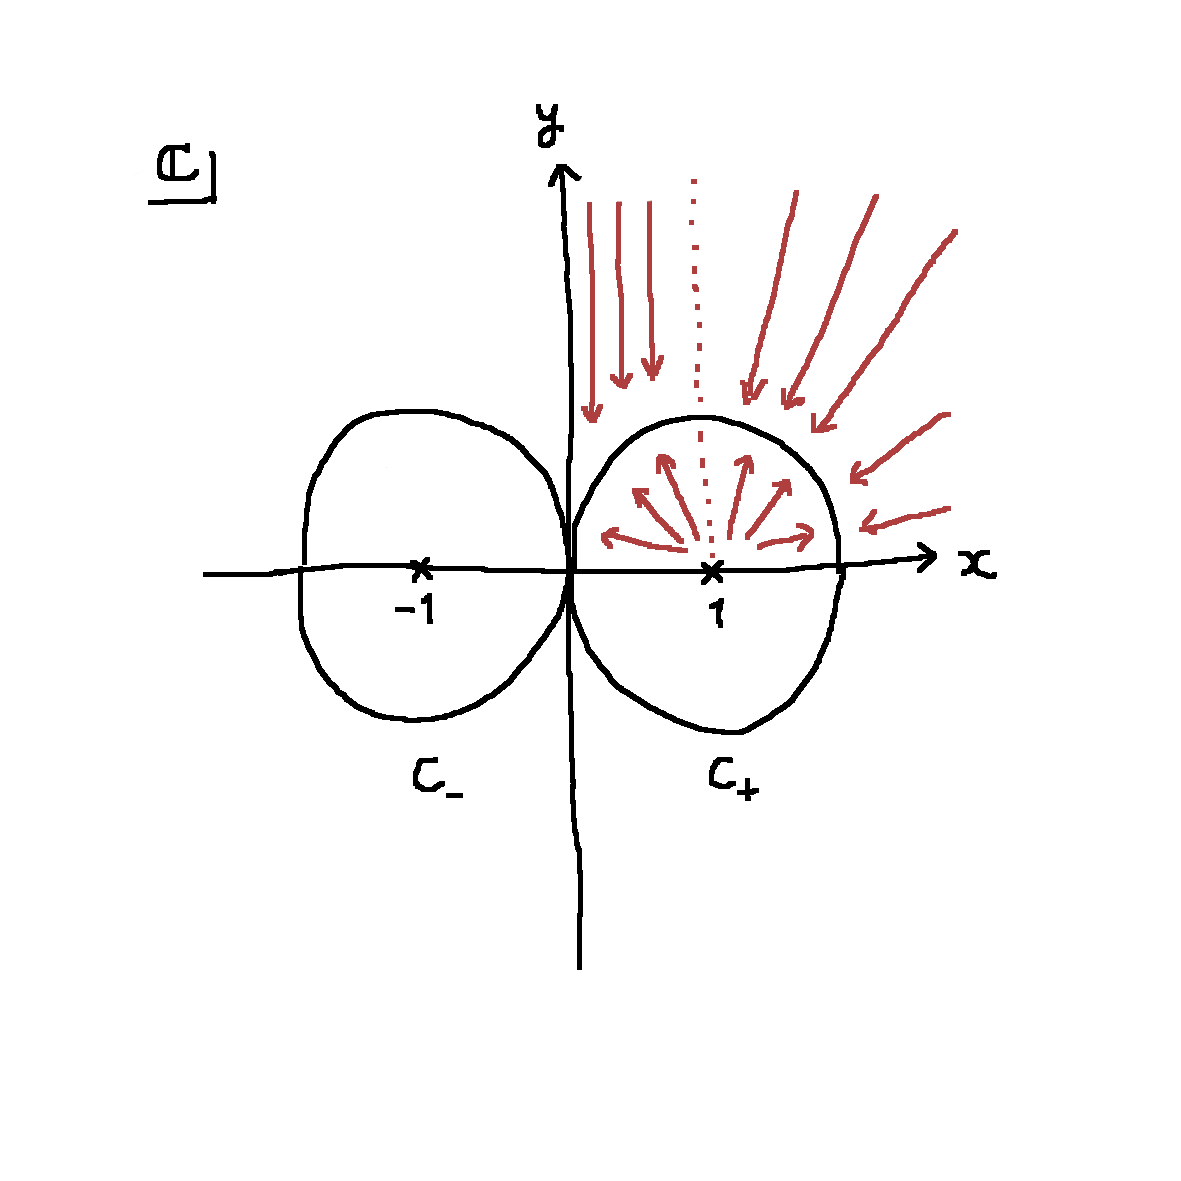
\includegraphics[width=8cm]{\assetspath assets/figure-eight.png}
    \caption{8の字空間}
    \label[figure]{fig:figure-eight}
\end{figure}





% ------------------------------------------------------------
%
% ------------------------------------------------------------
\section{被覆空間}

\TODO{連結性に関する仮定があやしいので書き直したい}

位相空間の被覆空間とは、
大まかには位相空間を局所的な形を保ったまま覆うような位相空間のことである。

\TODO{ファイバー束の特別な場合であることを強調すべき?}

\begin{definition}[被覆空間]
    $E, X$を位相空間とする。
    連続写像$p \colon E \to X$が次を満たすとき、
    $E$は\term{被覆空間}[covering space]{被覆空間}[ひふくくうかん]であるという:
    \begin{enumerate}
        \item $E$は連結かつ局所弧状連結である\footnote{
            したがってとくに弧状連結でもある。
        }。
        \item 各$x \in X$は$p$により
            \term{自明に被覆される}[trivially covered]{自明に被覆される}[じめいにひふくされる]
            近傍をもつ。すなわち、
            各$x \in X$に対し、
            $x \in \exists U \stackrel{\text{open}}{\subset} X$と
            $E$の disjoint な開集合の族
            $\exists \{ V_\lambda \}_{\lambda \in \Lambda}$が存在して
            次が成り立つ:
            \begin{enumerate}
                \item $p^{-1}(U)$は
                    \begin{equation}
                        p^{-1}(U) = \bigcup_{\lambda \in \Lambda} V_\lambda
                    \end{equation}
                    をみたす。
                \item 各$\lambda$に対し
                    $p|_{V_\lambda}$は$U$の上への同相写像である。
            \end{enumerate}
    \end{enumerate}
    このとき、
    \begin{itemize}
        \item $X$を\term{底空間}[base space]{底空間}[ていくうかん]、
        \item $U$を$x$の\term{自明化近傍}{自明化近傍}[じめいかきんぼう]、
        \item $V_\lambda$らを$U$上の$p$の\term{シート}[sheets]{シート}、
        \item $p^{-1}(x)$を$x$上の$p$の\term{ファイバー}[fiber]{ファイバー}
    \end{itemize}
    という(\cref{fig:covering-space-1})。
\end{definition}

\begin{figure}[t]
    \centering
    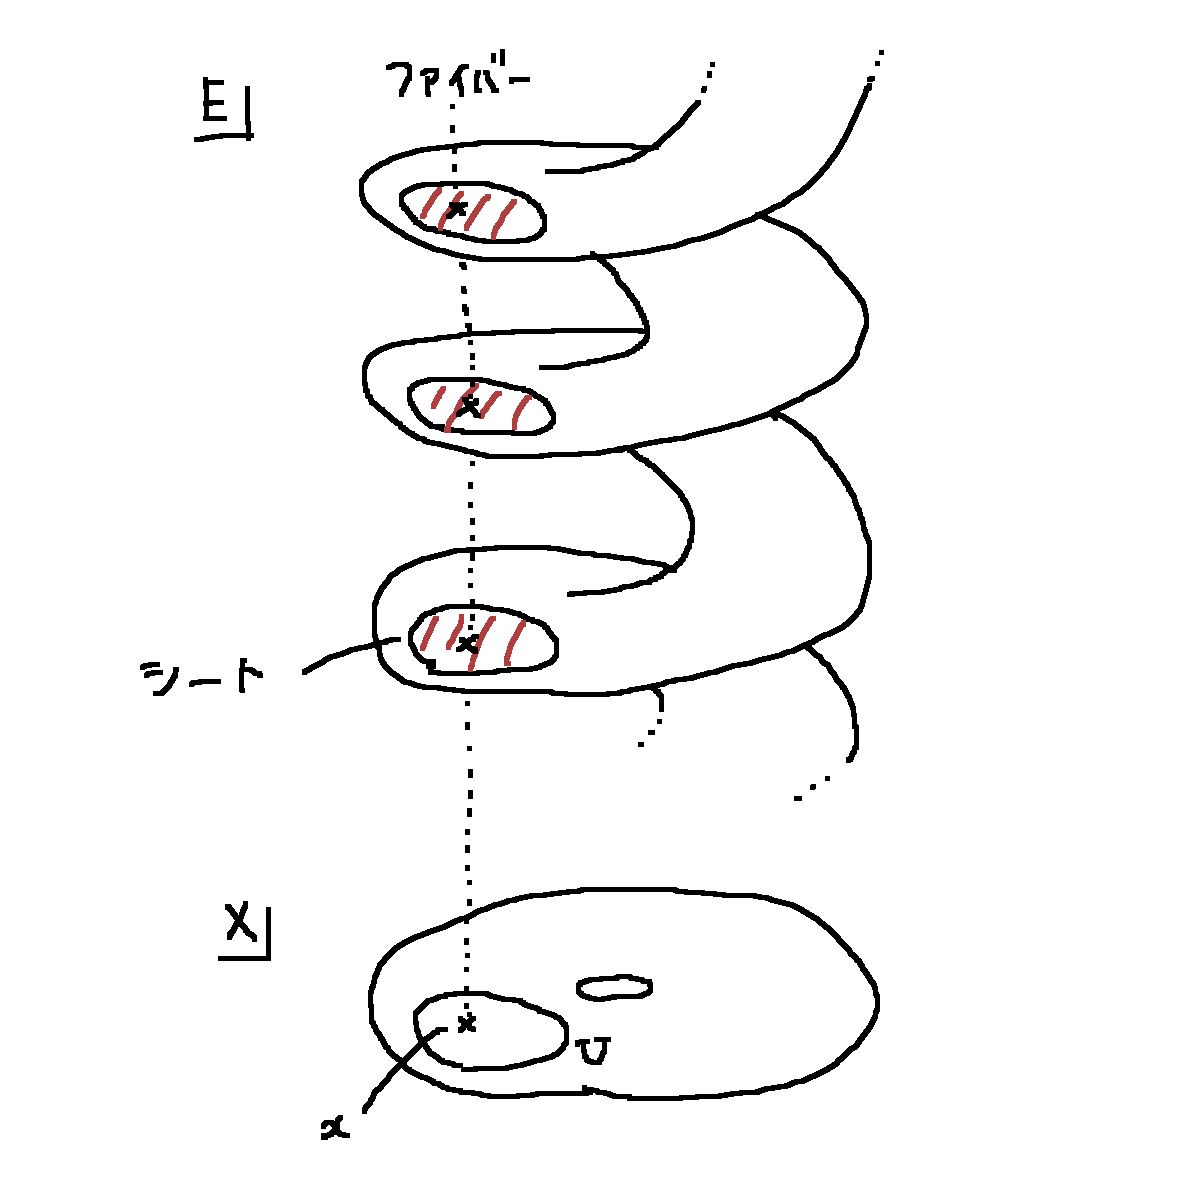
\includegraphics[width=8cm]{\assetspath assets/covering-space-1.png}
    \caption{被覆空間}
    \label[figure]{fig:covering-space-1}
\end{figure}

\begin{example}[被覆空間の例]
    ~
    \begin{itemize}
        \item $X$を位相空間とする。恒等写像$1_X \colon X \to X$は
            $X$の自明な被覆空間である。
    \end{itemize}
\end{example}

\begin{example}[$S^1$の被覆空間]
    \label[example]{ex:covering-space}
    $\R$は$S^1$の被覆空間である(\cref{fig:s1-covering-space-1})。
    被覆空間$p \colon \R \to S^1$は
    $p(x) \coloneqq e^{2\pi i x}$とおけばよいことを確かめる。
    $\delta > 0$を十分小さく固定しておく。
    各$z = e^{i\theta_0} \in S^1, 0 \le \theta_0 < 2\pi$に対し、
    $U \coloneqq \{ e^{i\theta}
        \in S^1 \colon \theta_0 - \delta < \theta < \theta_0 + \delta \}$とおけば、
    $U$は$S^1$における$z$の開近傍である。$U$は
    \begin{equation}
        p^{-1}(U) = \bigcup_{n \in \Z}
            \left(\theta_0 - \delta + 2n\pi, \theta_0 + \delta + 2n\pi\right)
    \end{equation}
    をみたし、各項は$p$により$U$と同相である。
    したがって、$U$は$p$により自明に被覆されることがわかる。
\end{example}

\begin{figure}[t]
    \centering
    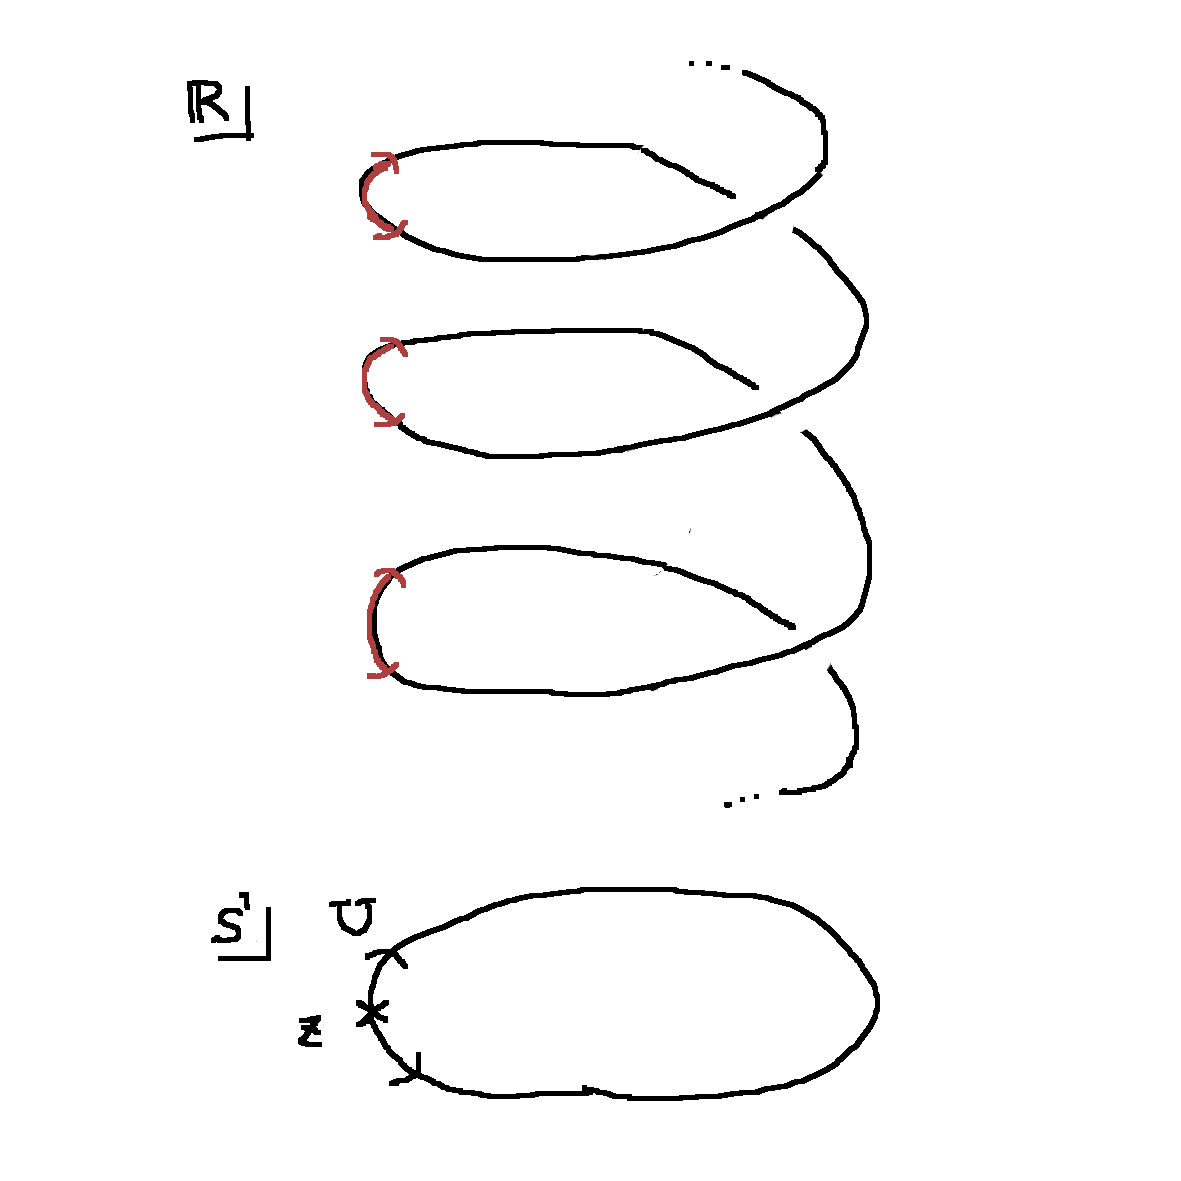
\includegraphics[width=8cm]{\assetspath assets/s1-covering-space-1.png}
    \caption{$S^1$の被覆空間}
    \label[figure]{fig:s1-covering-space-1}
\end{figure}

\begin{proposition}[ファイバーは離散空間]
    $p \colon E \to X$を被覆空間とする。
    このとき、各$x \in X$に対しファイバー$p^{-1}(x)$は離散空間である。
\end{proposition}

\begin{proof}
    各$e \in p^{-1}(x)$に対し$\{e\}$が$p^{-1}(x)$の開集合であることをいえばよい。
    そこで$x$の自明化近傍$U$をひとつ固定すると、
    $U$上のシート$V_\lambda$であって$e$の属するものがただひとつ存在する。
    $\{e\} = V_\lambda \cap p^{-1}(x)$を示せばよい。
    右向きの包含は明らかだから、逆向きを示す。
    そこで$e' \in V_\lambda \cap p^{-1}(x)$とすると、
    $p(e') = x = p(e)$であるが、
    $p$は$V_\lambda$から$U$への単射だから$e' = e$、
    したがって$e' \in \{e\}$である。
    よって逆向きの包含もいえた。
\end{proof}

被覆空間は全射連続開写像である。

\begin{proposition}[被覆空間は全射連続開写像]
    \TODO{}
\end{proposition}

\begin{proof}
    \TODO{}
\end{proof}

\subsection{リフト}

リフトについて述べる。

\TODO{多価関数の枝についての例を念頭に考えたい}

\begin{definition}[リフト]
    $p \colon E \to X$を被覆空間、
    $f \colon Y \to X$を連続写像とする。
    連続写像$\wt{f} \colon Y \to E$が
    $p$による$f$の
    \term{リフト}[lift]{リフト}
    あるいは\term{持ち上げ}{持ち上げ}[もちあげ]
    であるとは、図式
    \begin{equation}
        \begin{tikzcd}
            & E \ar{d}{p} \\
            Y \ar[dashed]{ur}{\wt{f}} \ar{r}[swap]{f} & X
        \end{tikzcd}
    \end{equation}
    が可換となることをいう(\cref{fig:lift-1})。
\end{definition}

\begin{figure}[t]
    \centering
    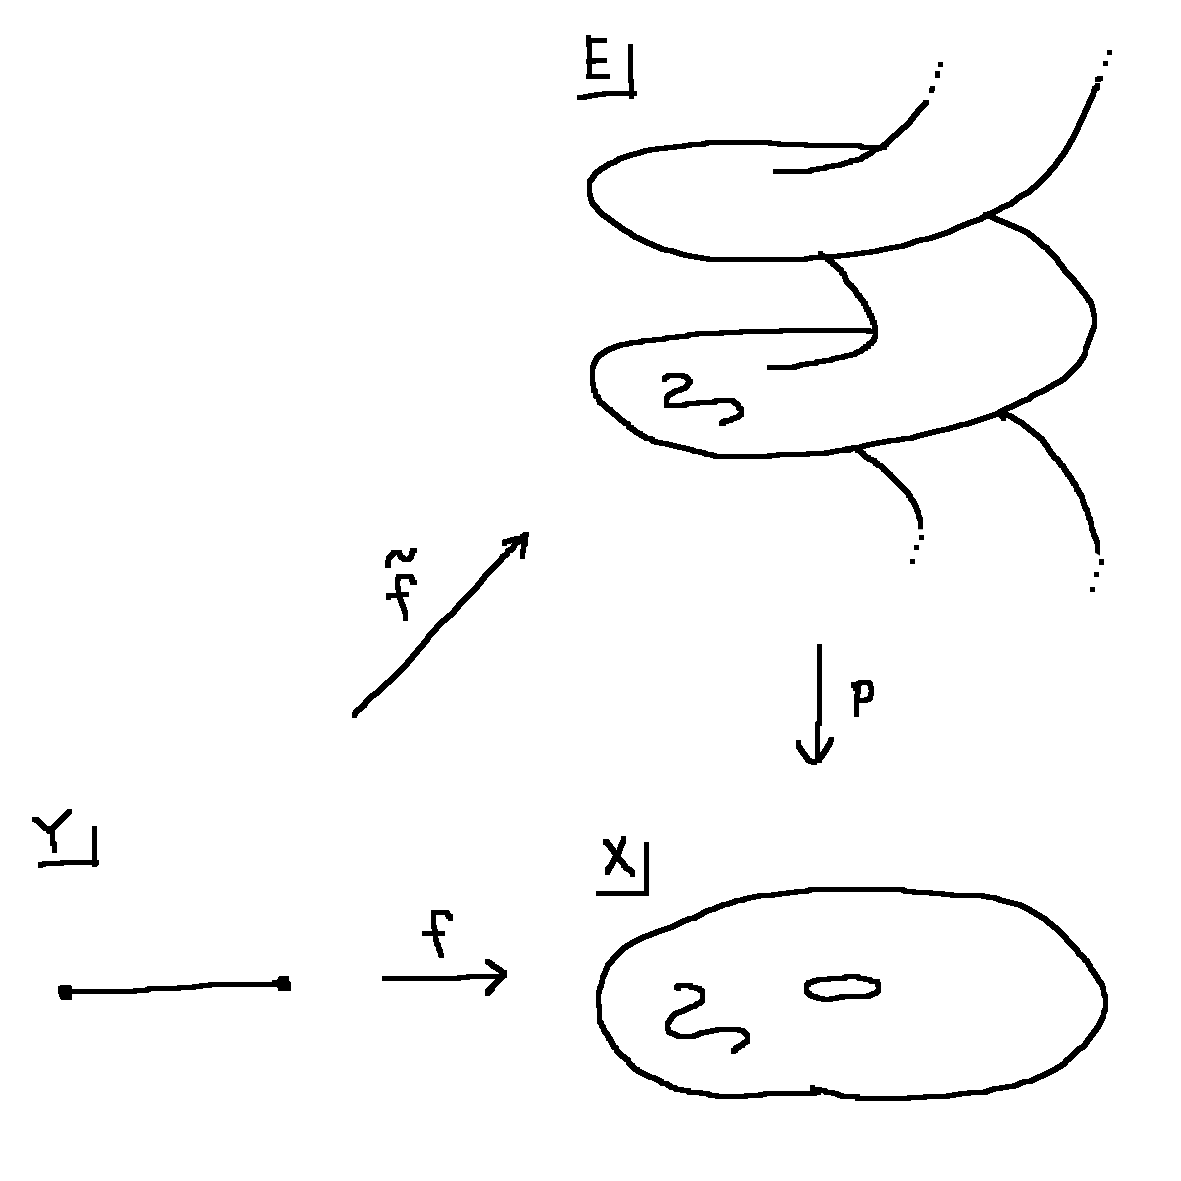
\includegraphics[width=8cm]{\assetspath assets/lift-1.png}
    \caption{リフト}
    \label[figure]{fig:lift-1}
\end{figure}

\begin{example}[リフトが存在しない例]
    \cref{ex:covering-space}の被覆空間$p \colon \R \to S^1$を考える。
    $f \colon S^1 \to S^1$を恒等写像とすると、
    $p$による$f$のリフト$\wt{f}$は存在しない。
    \begin{equation}
        \begin{tikzcd}
            & \R \ar[d, "{p}"] \\
            S^1 \ar[ur, dashed, "{\wt{f}}"] \ar[r, "{f}"'] & S^1
        \end{tikzcd}
    \end{equation}
    実際、もしこのようなリフト$\wt{f}$が存在するとしたら、
    $p \circ \wt{f}$から誘導される群準同型
    $(p \circ \wt{f})_* \colon \pi_1(S^1) \to \pi_1(S^1)$
    は恒等写像となるから、$p_* \colon \pi_1(\R) \to \pi_1(S^1)$は全射である。
    ところが、($S^1$が単連結でないことを認めると)
    $\pi_1(S^1)$は非自明で$\pi_1(\R)$は自明だからこれは矛盾である。
    したがって上のようなリフト$\wt{f}$は存在しない。
\end{example}

\begin{example}[リフトが一意でない例]
    $U \subset \C^\times$を単連結領域とする。
    このとき、指数関数$\exp \colon \C \to \C^\times,\;
    z \mapsto \exp(z)$は被覆空間である。
    また、各$n_0 \in \Z$に対し
    写像$\log_{n_0} \colon U \to \C,\;
    z \mapsto \log |z| + i (\mathrm{Arg} (z) + 2n_0\pi)$
    は$\exp$による$f \colon U \to \C^\times,\; z \mapsto z$のリフトである。
    $n_0$をどのようにとっても$\log_{n_0}$は$\exp$のリフトであるが、
    $\log_{n_0}$は$n_0$ごとに異なるから、
    リフトは一意的でないことが確かめられた。
    \begin{equation}
        \begin{tikzcd}
            & \C \ar{d}{\exp} \\
            U \ar{ur}{\log_{n_0}} \ar{r}[swap]{\id_{U}} & C^\times
        \end{tikzcd}
    \end{equation}
\end{example}

連結空間 (たとえば$I$) からの写像がリフトを持つとき、
上の例で見たようにそれは一意とは限らないが、
1点での値を決めれば一意に定まる。
証明の手法は連結性を用いる典型的なものである。

\begin{theorem}[リフトの一意性定理]
    $p \colon E \to X$を被覆空間、
    $Y$を\highlight{連結}位相空間、
    $\varphi \colon Y \to X$を連続写像とする。
    $\wt{\varphi}_1, \wt{\varphi}_2 \colon Y \to E$を
    $p$による$\varphi$のリフトとするとき、
    $\wt{\varphi}_1, \wt{\varphi}_2$が
    1点で一致するならば全体で一致する。
\end{theorem}

\begin{proof}
    $B \coloneqq \{ x \in Y \colon \wt{\varphi}_1(x) = \wt{\varphi}_2(x) \}$
    とおく。問題の仮定より$B$は空でない。
    $Y$は連結だから、$B$が$Y$で開かつ閉であることを示せば$B = Y$となり定理の主張が従う。
    \begin{equation}
        \begin{tikzcd}[row sep=huge, column sep=huge]
            & E \ar[d, "{p}"] \\
            Y \ar[ur, shift left, "{\wt{\varphi}_1}"]
                \ar[ur, shift right, "{\wt{\varphi}_2}"'] \ar[r, "{\varphi}"'] & X
        \end{tikzcd}
    \end{equation}

    \noindent
    \uline{$B$が$Y$で開であること} \quad
    $b_0 \in B$とする。
    \begin{equation}
        e \coloneqq \wt{\varphi}_1(b_0) = \wt{\varphi}_2(b_0),
        \quad
        x_0 \coloneqq \varphi(b_0) = p(e)
    \end{equation}
    とおく。
    $x_0$の自明化近傍$U \subset X$と、
    $U$上のシート$\wt{U}$であって$e$を含むものが存在する。
    ここで
    $V \coloneqq \wt{\varphi}_1^{-1}(\wt{U})
        \cap \wt{\varphi}_2^{-1}(\wt{U})$
    とおくと、
    $V$は$Y$における$b_0$の開近傍であり、
    $\wt{\varphi}_1, \wt{\varphi}_2$は$V$上で$\wt{U}$に値をとる。
    したがって
    \begin{itemize}
        \item $\varphi$は$V \to U$の連続写像とみなすことができ、
        \item $\wt{\varphi}_1, \wt{\varphi}_2$は
            $V \to \wt{U}$の連続写像とみなすことができ、
        \item $p$は$\wt{U} \to U$の同相写像とみなすことができる。
    \end{itemize}
    よって、図式
    \begin{equation}
        \begin{tikzcd}[row sep=huge, column sep=huge]
            & \wt{U} \ar{d}{p}[swap, anchor=center, rotate=90, yshift=1ex]{\approx} \\
            V \ar[shift left]{ur}{\wt{\varphi}_1}
                \ar[shift right]{ur}[swap]{\wt{\varphi}_2}
                \ar[r, "{\varphi}"']
                & U
        \end{tikzcd}
    \end{equation}
    は可換となる。$p$の$\wt{U}$上での単射性から
    $V$上$\wt{\varphi}_1 = \wt{\varphi}_2$となることがわかる。
    したがって$b_0 \in V \subset B$であり、$b_0$は$Y$における$B$の内点であることがいえた。
    $b_0 \in B$は任意であったから、$B$は$Y$で開である。

    \noindent
    \uline{$B$が$Y$で閉であること} \quad
    $Y \setminus B$が$Y$で開であることを示す。
    $b_0 \in Y \setminus B$とする。
    $e_1 \coloneqq \wt{\varphi}_1(b_0),\;
    e_2 \coloneqq \wt{\varphi}_2(b_0)$とおくと、
    $b_0 \not\in B$より$e_1 \neq e_2$である。
    $x_0 \coloneqq p(e_1) = p(e_2) = \varphi(b_0)$とおくと、
    $x_0$の自明化近傍$U \subset X$と、
    $U$上のシート$\wt{U}_1, \wt{U}_2$であって
    $e_1, e_2$をそれぞれ含むものが存在する。
    このとき$\wt{U}_1 \cap \wt{U}_2 = \emptyset$である
    \begin{innerproof}
        もし交わりをもったとすれば、シートの disjoint 性より
        $\wt{U}_1 = \wt{U}_2$でなければならないが、
        すると$p$が$\wt{U}_1 = \wt{U}_2$から$U$への全単射となることから
        $e_1 = (p|_{\wt{U}_1})^{-1}(x_0)
        = (p|_{\wt{U}_2})^{-1}(x_0) = e_2$となり矛盾。
    \end{innerproof}
    ここで$V \coloneqq \wt{\varphi}_1^{-1}(\wt{U}_1)
    \cap \wt{\varphi}_2^{-1}(\wt{U}_2)$とおくと、
    $V$は$Y$における$b_0$の近傍であり、
    $\wt{\varphi}_1(V) \subset \wt{U}_1,\;
    \wt{\varphi}_2(V) \subset \wt{U}_2$をみたす。
    よって$V$上$\wt{\varphi}_1 \neq \wt{\varphi}_2$である。
    したがって$V \subset Y \setminus B$であり、
    $b_0$は$Y$における$Y \setminus B$の内点であることがいえた。
    $b_0 \in Y \setminus B$は任意であったから、
    $Y \setminus B$は$Y$で開である。
    よって$B$は$Y$で閉である。
\end{proof}

リフトの存在について調べる。
まずは一般の写像のリフトではなく
パスのリフトに限って考えよう。
パスのリフトの存在に関する定理はすべて次の定理から導かれる。

\begin{theorem}[被覆ホモトピー定理]
    $p \colon E \to X$を被覆空間、
    $Y$を位相空間とする。
    このとき、図式
    \begin{equation}
        \begin{tikzcd}
            Y
                \ar{r}{\wt{f}}
                \ar{d}[swap]{y \mapsto (y, 0)}
                & E
                    \ar{d}{p} \\
            Y \times I
                \ar[dashed]{ru}{\wt{F}}
                \ar{r}[swap]{F}
                & X
        \end{tikzcd}
    \end{equation}
    を可換にする$\wt{F}$が一意に存在する。
\end{theorem}

\begin{proof}
    \TODO{}
\end{proof}

\begin{corollary}[パスのリフトの一意存在定理]
    $p \colon E \to X$を被覆空間、
    $\gamma \colon I \to X$をパス、
    $e \in p^{-1}(\gamma(0))$とする。
    このとき、$p$による$\gamma$のリフト
    $\wt{\gamma} \colon I \to E$であって
    $\wt{\gamma}(0) = e$を満たすものが一意に存在する。
\end{corollary}

\begin{proof}
    \TODO{}
\end{proof}

\begin{corollary}[モノドロミー定理]
    \termhidden[monodoromy theorem]{モノドロミー定理}[ものどろみーていり]
    $p \colon E \to X$を被覆空間、
    $f, g \colon I \to X$を
    点$x_0$から$x_1$へのパス、
    $\wt{x}_0 \in p^{-1}(x_0)$とする。
    \begin{enumerate}
        \item (パスのホモトピーのリフトの一意存在) \quad
            $H \colon f \sim g \; \rel \; \{ 0, 1 \}$ならば、
            $H$のリフト$\wt{H} \colon I \times I \to E$であって
            $\wt{H}(0, 0) = \wt{x}_0$を満たすものが一意に存在する。
        \item (モノドロミー定理) さらに
            $\wt{x}_0$を始点とする
            $f, g$のリフトをそれぞれ
            $\wt{f}, \wt{g}$とおくと、
            $\wt{f}$と$\wt{g}$は終点も一致し、
            さらに
            $\wt{H} \colon f \sim g \; \rel \; \{ 0, 1 \}$
            が成り立つ。
    \end{enumerate}
\end{corollary}

\begin{proof}
    \TODO{}
\end{proof}

モノドロミー定理を用いて
$S^1$は単連結でないことを示そう。

\begin{theorem}
    $S^1$は単連結でない。
\end{theorem}

\begin{proof}
    写像$p \colon \R \to S^1, \;
        t \mapsto \exp(2\pi i t)$
    は$S^1$の被覆空間である。
    ここで写像$\gamma, \wt{\gamma}$を
    \begin{alignat}{1}
        \gamma \colon I \to S^1, \quad & t \mapsto \exp(2\pi i t) \\
        \wt{\gamma} \colon I \to \R, \quad & t \mapsto t
    \end{alignat}
    で定めると、$\wt{\gamma}$は$\gamma$のリフトである。
    また、写像$\beta$を
    \begin{alignat}{1}
        \beta \colon I \to S^1, \quad & t \mapsto 1 \\
        \wt{\beta} \colon I \to \R, \quad & t \mapsto 0
    \end{alignat}
    で定めると、$\wt{\beta}$は$\beta$のリフトである。
    ここで$S^1$が単連結であると仮定すると、
    $\beta$と$\gamma$が共通の端点を持つことから
    \begin{equation}
        H \colon \beta \sim \gamma \quad \rel \quad \{ 0, 1 \}
    \end{equation}
    が成り立つ。
    $\wt{\beta}, \wt{\gamma}$は共通の始点を持つから
    モノドロミー定理より終点も共通である。
    ところが定義より$\wt{\beta}(1) = 0 \neq 1 = \wt{\gamma}(1)$だから矛盾。
    したがって$S^1$は単連結でない。
\end{proof}

次に写像のリフトの存在について考える。
一般の写像の定義域はパスの定義域$I$のように良い性質を持つとは限らない。
そこで定義域の連結性を限定したクラスのなかで存在条件を考えることになる。

\begin{theorem}[リフトの存在条件]
    $p \colon E \to X$を被覆空間、
    $Y$を\highlight{連結かつ局所弧状連結}な位相空間、
    $f \colon (Y, y_0) \to (X, x_0)$を連続写像、
    $\wt{x}_0 \in p^{-1}(x_0)$とする。
    このとき、次は同値である:
    \begin{enumerate}
        \item $f$のリフト$\wt{f} \colon (Y, y_0) \to (E, \wt{x}_0)$が一意に存在する。
        \item $f_* \pi_1(Y, y_0) \subset p_* \pi_1(E, \wt{x}_0)$である。
    \end{enumerate}
\end{theorem}

\begin{proof}
    $Y$は連結なので一意性は成り立つ。

    \TODO{}
\end{proof}



\subsection{ファイバーへの基本群の作用}

位相空間の基本群は、被覆空間のファイバーへの自然な群作用をもつ。

\TODO{}

%\begin{theorem}[モノドロミー作用の well-defined 性]
%    \label[theorem]{thm:monodromy-well-defined}
%    $p \colon E \to X$を被覆空間とし、$x \in X$とする。
%    このとき、基本群$\pi_1(X, x)$の$p^{-1}(x)$への右作用が
%    \begin{equation}
%        e \cdot [f] \coloneqq \tilde{f}_e(1) \quad (\forall e \in p^{-1}(x), [f] \in \pi_1(X, x))
%    \end{equation}
%    により定まる。
%    この作用を\term{モノドロミー作用}[monodromy action]{モノドロミー作用}という
%    (\cref{fig:monodromy-1})。
%\end{theorem}
%
%\begin{figure}[t]
%    \centering
%    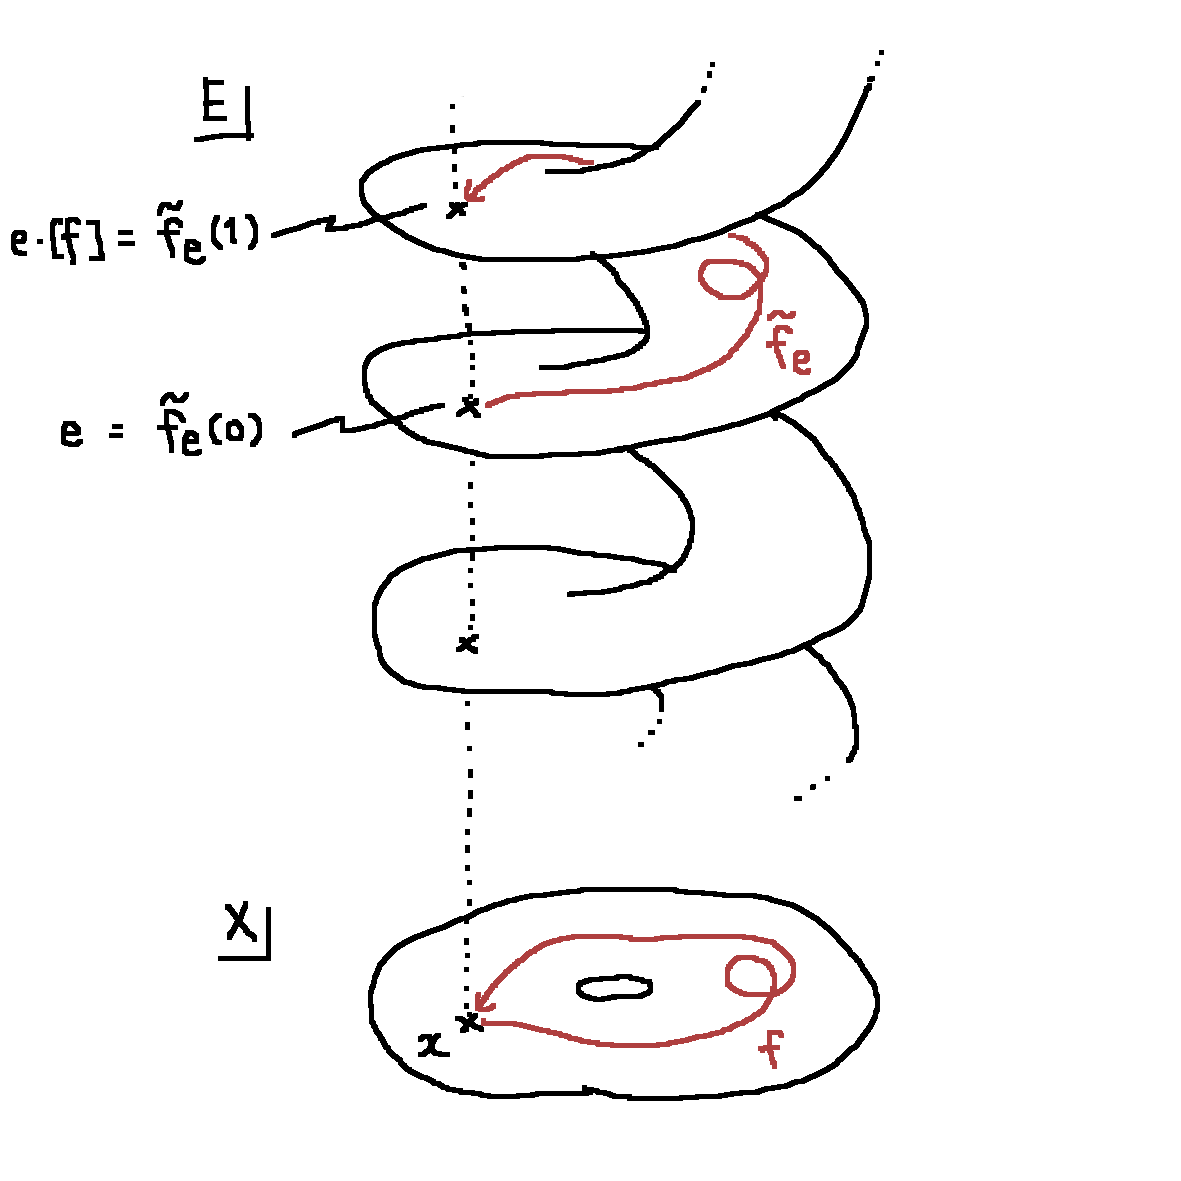
\includegraphics[width=8cm]{\assetspath assets/monodromy-1.png}
%    \caption{モノドロミー作用}
%    \label[figure]{fig:monodromy-1}
%\end{figure}
%
%\begin{proof}
%    省略
%\end{proof}
%
%\begin{remark}[モノドロミー作用の不動点]
%    すぐわかるように、$f$を$X$内のパスとするとき、
%    $e \cdot [f] = e$であることと
%    $\tilde{f}_e$が$e$を基点とするループであることとは同値である。
%\end{remark}
%
%\begin{theorem}[弧状連結な被覆空間のモノドロミー作用]
%    \label[theorem]{thm:monodromy-path-connected}
%    \cref{thm:monodromy-well-defined}の状況でさらに$E$が弧状連結ならば、モノドロミー作用は推移的である。
%
%    \TODO{被覆空間は定義より弧状連結なのでは?}
%\end{theorem}
%
%\begin{proof}
%    省略
%\end{proof}
%
%\begin{theorem}[モノドロミー作用の固定部分群]
%    \label[theorem]{thm:monodromy-stabilizer}
%    $p \colon E \to X$を被覆空間、$x \in X$とし、$E$は弧状連結であるとする。
%    このとき、各$e \in p^{-1}(x)$に対し、
%    モノドロミー作用に関する$e$の固定部分群は$p_* (\pi_1(E, e)) \subseteq \pi_1(X, x)$で与えられる。
%\end{theorem}
%
%\begin{proof}
%    省略
%\end{proof}
%
%\TODO{普遍被覆を導入したあとで述べるべき?}
%
%\begin{corollary}[単連結な被覆空間のモノドロミー作用]
%    \label[theorem]{thm:monodromy-simply-connected}
%    $p \colon E \to X$を被覆空間とし、$E$は単連結であるとする。
%    このとき、各ファイバーへのモノドロミー作用は自由である。
%\end{corollary}
%
%\begin{proof}
%    $x \in X$を任意に固定する。
%    $\pi_1(X, x)$の$p^{-1}(x)$へのモノドロミー作用が自由であることは、
%    作用に関する固定部分群がすべて自明であることと同値であり、
%    さらに\cref{thm:monodromy-stabilizer}より、これはすべての$e \in p^{-1}(x)$に対し
%    $p_* (\pi_1(E, e))$が自明であることと同値である。
%    そこで、各$e \in p^{-1}(x)$に対し$p_* (\pi_1(E, e))$が自明であることを示す。
%    系の仮定より$E$は単連結だから、$\pi_1(E, e)$は自明である。
%    したがって$p_* (\pi_1(E, e))$も自明である。
%\end{proof}

\subsection{普遍被覆}

単連結な被覆空間を普遍被覆という。

\begin{definition}[普遍被覆]
    被覆空間$p \colon E \to X$が単連結であるとき、
    $p$を\term{普遍被覆}[universal covering]{普遍被覆}[ふへんひふく]という。
\end{definition}

普遍被覆は存在すれば次の定理の意味で一意である。
したがって$X$が単連結ならば
$X$自身が (自明な被覆として) 普遍被覆となる。

\begin{theorem}[普遍被覆の一意性]
    普遍被覆は被覆空間としての同型を除いて一意である。
    \TODO{}
\end{theorem}

\begin{proof}
    \TODO{}
\end{proof}

普遍被覆はつねに存在するとは限らない。
存在条件は次の定理で与えられる。

\begin{theorem}[普遍被覆の存在定理]
    半局所単連結であること
    \TODO{}
\end{theorem}

\begin{proof}
    \TODO{}
\end{proof}

\begin{proposition}[普遍被覆のファイバーと基本群]
    $X$を位相空間、$p \colon \wt{X} \to X$を普遍被覆とし、
    $p$は$\wt{x}_0 \in \wt{X}$を$x_0 \in X$に写すとする。
    このとき、写像
    \begin{equation}
        \pi_1(X, x_0) \to p^{-1}(x_0),
        \quad
        [\gamma] \mapsto \wt{\gamma}(1)
    \end{equation}
    は全単射である。ただし、$\wt{\gamma}$は$\wt{x}_0$を始点とする
    $\gamma$のリフトである。
    また、逆写像は$y \in p^{-1}(x_0)$に対し
    $\wt{x}_0$を$y$につなぐパス$\beta$をひとつ選んで
    $[p \circ \beta]$を対応付けることで得られる。
\end{proposition}

\begin{proof}
    \TODO{}
\end{proof}

\subsection{被覆変換群}

被覆空間の射と被覆変換群について述べる。

\begin{definition}[被覆空間の射]
    $p \colon E \to X, \; p' \colon E' \to X$を被覆空間とする。
    連続写像$f \colon E \to E'$であって
    \begin{equation}
        \begin{tikzcd}
            E \ar{rr}{f} \ar{rd}[swap]{p}
                && E' \ar{ld}{p'} \\
            & X
        \end{tikzcd}
    \end{equation}
    を可換にするものを
    \term{被覆空間の射}[morphism of covering spaces]
        {被覆空間の射}[ひふくくうかんのしゃ]
    という。
\end{definition}

\begin{definition}[被覆変換群]
    \idxsym{covering transformation group}{$\Deck(E)$}{被覆空間$E$の被覆変換群}
    被覆空間の自己同型射を
    \term{被覆変換}[covering transformation]
        {被覆変換}[ひふくへんかん]
    という。
    被覆空間$E$の被覆変換全体のなす群を
    $\Deck(E)$と書き、
    $E$の\term{被覆変換群}[covering transformation group]
        {被覆変換群}[ひふくへんかんぐん]
    という。
\end{definition}

普遍被覆の被覆変換群は基本群の計算に利用できる。

\begin{theorem}[普遍被覆の被覆変換群と基本群]
    $X$を局所弧状連結な位相空間、
    $p \colon \wt{X} \to X$を普遍被覆とする。
    このとき、任意の$x_0 \in X$に対し群の同型
    \begin{equation}
        \pi_1(X, x_0) \cong \Deck(\wt{X})
    \end{equation}
    が成り立つ。
\end{theorem}

\begin{proof}
    \TODO{}
\end{proof}


% ------------------------------------------------------------
%
% ------------------------------------------------------------
\section{
    \texorpdfstring{%
        $S^1$の基本群%
    }{%
        S1の基本群%
    }%
}

$S^1$の基本群を計算する。
$S^1$の基本群は最も身近にある非自明な例というばかりでなく、
ホモロジーの理論の基礎にもつながっている。
\TODO{どのように?}

\begin{lemma}[$S^1$のループのリフト]
    \label[lemma]{lem:s1-loop-lift}
    \cref{ex:covering-space}の被覆空間$p \colon \R \to S^1$を考える。
    ここだけの用語として、
    各$k \in \Z$に対し、$S^1$上を点$1$から反時計回りに$k$周するループ
    \begin{equation}
        \omega_k \colon I \to S^1, \quad t \mapsto e^{2\pi kit}
    \end{equation}
    を\emph{$k$-基本ループ ($k$-elementary loop)}と呼ぶことにする。
    \TODO{必要ある?}
    このとき、$0 \in \R$を始点とする$\omega_k$のリフト
    $(\tilde{\omega}_k)_0$は
    \begin{equation}
        (\tilde{\omega}_k)_0 \colon I \to \R, \quad t \mapsto kt
    \end{equation}
    で与えられる。
\end{lemma}

\begin{proof}
    補題の$(\tilde{\omega}_k)_0$は
    \begin{equation}
        \begin{tikzcd}
            & \R \ar[d, "{p}"] \\
            I \ar[ur, "{(\tilde{\omega}_k)_0}"] \ar[r, "{\omega_k}"'] & S^1
        \end{tikzcd}
    \end{equation}
    を可換にする連続写像だから$\omega_k$のリフトであり、
    また明らかに始点は$0$である。
\end{proof}

\begin{theorem}[$S^1$の基本群]
    $\pi_1(S^1) \cong \Z$である(\cref{fig:s1-monodromy-1})。
\end{theorem}

\begin{figure}[t]
    \centering
    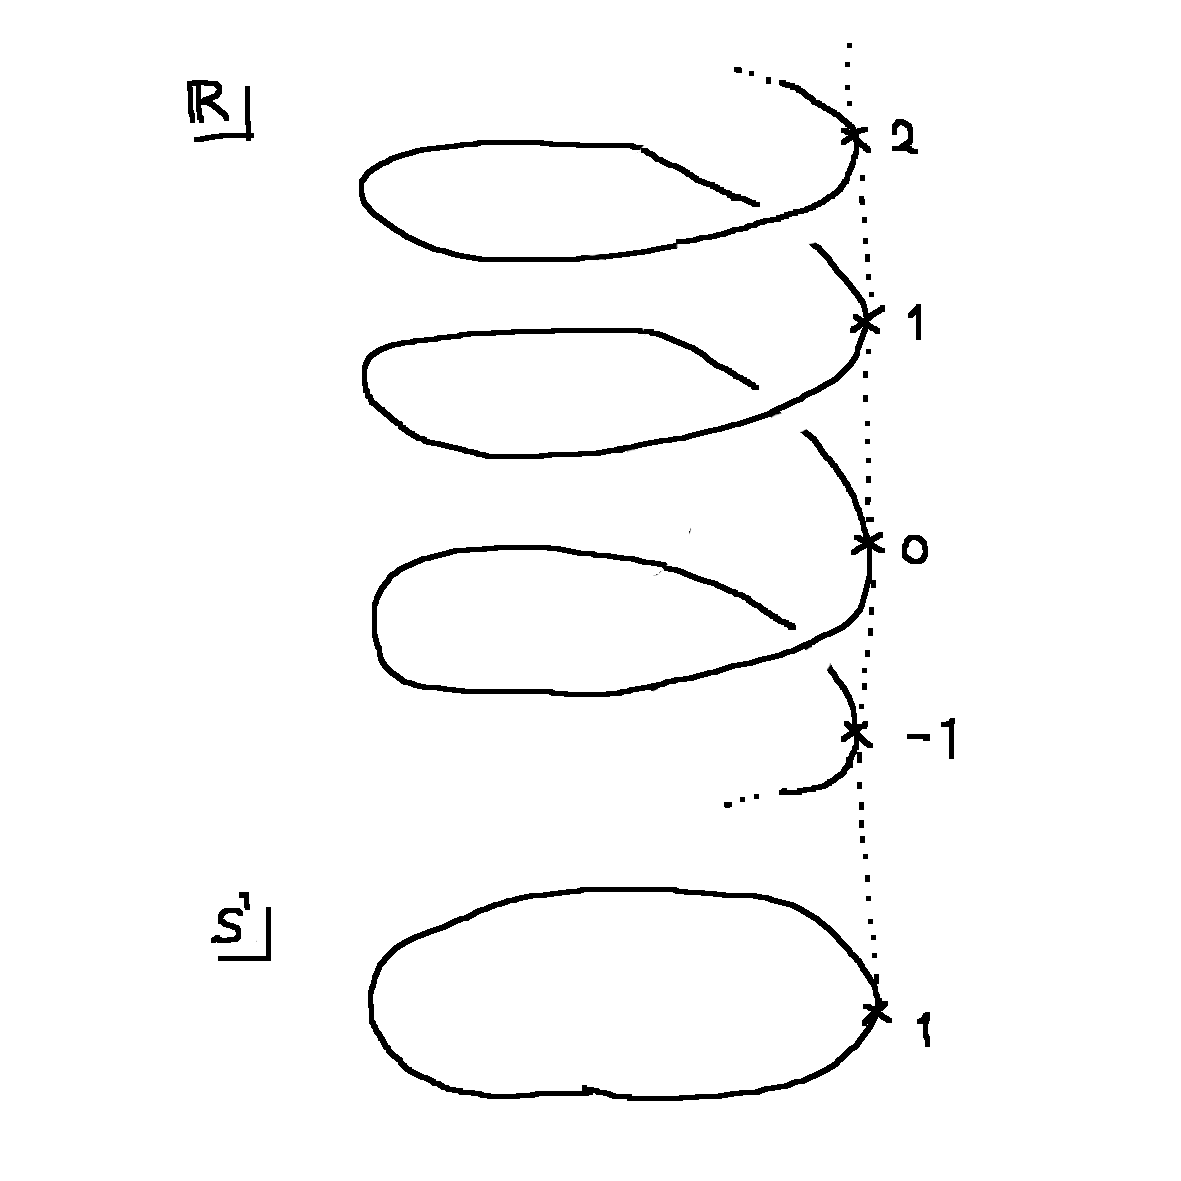
\includegraphics[width=8cm]{\assetspath assets/s1-monodromy-1.png}
    \caption{$S^1$の基本群}
    \label[figure]{fig:s1-monodromy-1}
\end{figure}

\begin{proof}
    \cref{ex:covering-space}の被覆空間$p \colon \R \to S^1$を考える。
    $\R$は単連結だから、\cref{thm:monodromy-path-connected}および\cref{thm:monodromy-simply-connected}より
    $\pi_1(S^1, 1)$の$p^{-1}(1)$へのモノドロミー作用は推移的かつ自由である。
    したがって、写像$\Phi \colon \pi_1(S^1, 1) \to p^{-1}(1),$
    \begin{equation}
        [f] \mapsto 0 \cdot [f]
    \end{equation}
    は全単射である。
    \begin{innerproof}
        \uline{全射性}\; 作用が推移的であることの定義から明らか。\\
        \uline{単射性}\; $[f], [g] \in \pi_1(S^1, 1)$とする。
            \begin{alignat}{1}
                \Phi([f]) = \Phi([g]) 
                    &\Rightarrow 0 \cdot [f] = 0 \cdot [g] \\
                    &\Rightarrow 0 \cdot ([f] \cdot [g]^{-1}) = 0 \\
                    &\Rightarrow [f] \cdot [g]^{-1} = 1 \quad (\because \text{ 作用は自由}) \\
                    &\Rightarrow [f] = [g]
            \end{alignat}
            より、単射性がいえた。
    \end{innerproof}

    あとは$\Phi$が群準同型であることをいえばよい。
    そこで、まず$\pi_1(S^1, 1)$の具体的な形を考える。
    いま$p$の定め方から$p^{-1}(1) = \Z$であったから、
    $\pi_1(S^1, 1) = \Phi^{-1}(\Z)$である。
    $\Phi([\omega_k]) = 0 \cdot [\omega_k] = (\tilde{\omega}_k)_0(1) = k$ゆえに
    $\Phi^{-1}(k) = [\omega_k]$だから、
    \begin{equation}
        \pi_1(S^1, 1) = \Phi^{-1}(\Z) = \{ [\omega_k] \colon k \in \Z \}
    \end{equation}
    と表せることがわかる。

    $\Phi$が群準同型であることを示す。
    \begin{alignat}{1}
        \Phi([\omega_k] \cdot [\omega_j])
            &= 0 \cdot ([\omega_k] \cdot [\omega_j]) \\
            &= 0 \cdot [\omega_k * \omega_j] \\
            &= 0 \cdot [\omega_{k+j}] \\
            &= (\tilde{\omega}_{k+j})_0(1) \\
            &= k+j \quad (\cref{lem:s1-loop-lift}) \\
            &= (\tilde{\omega}_{k})_0(1) + (\tilde{\omega}_{j})_0(1) \quad (\cref{lem:s1-loop-lift}) \\
            &= 0 \cdot [\omega_{k}] + 0 \cdot [\omega_{j}] \\
            &= \Phi([\omega_k]) + \Phi([\omega_j])
    \end{alignat}
    だから、$\Phi$は$\Z$と$\pi_1(S^1, 1)$との群準同型であることがいえた。
    以上で$\pi_1(S^1) = \pi_1(S^1, 1) \cong \Z$がいえた。
\end{proof}

\begin{corollary}[トーラスの基本群]
    \label[corollary]{cor:torus-fundamental-group}
    $\pi_1(T^2) \cong \Z \times \Z$である。 
\end{corollary}

\begin{proof}
    \cref{ex:torus-fundamental-group}ですでに確かめた。
    また、\cref{problem:geometry2-4.2}で被覆変換群を用いる別解を与えた。
\end{proof}




% ------------------------------------------------------------
%
% ------------------------------------------------------------
\section{Seifert-Van Kampen の定理 \!${}^*$}

Seifert-Van Kampen の定理は、一定の条件下において、
位相空間の基本群が部分空間の基本群の融合積に分解できることを述べた定理である。
定理の系として、
wedge 和やCW複体の基本群が簡単に計算できるようになる。
ここでは wedge 和の例を計算する。


\begin{theorem}[Seifert-Van Kampen の定理]
    $X$を位相空間とする。$U, V \subset X$は開部分集合であって、
    $U \cup V = X$をみたし、$U, V, U \cap V$は弧状連結であるとする。
    $p \in U \cap V$とし、部分集合$C \subset \pi_1(U, p) * \pi_1(V, p)$を
    \begin{equation}
        C \coloneqq \{ (i_* \gamma)(j_* \gamma)^{-1} \colon \gamma \in \pi_1(U \cap V, p) \}
    \end{equation}
    で定義する。
    \TODO{}
\end{theorem}

\begin{proof}
    省略
\end{proof}

\begin{example}[円のブーケ]
    \TODO{}
\end{example}



% ------------------------------------------------------------
%
% ------------------------------------------------------------
\newpage
\section{演習問題}

\subsection{問題セット 2}

\begin{problem}[幾何学II 2.1]
    $\R^2 \setminus ((-\infty, 0] \times \{0\})$は可縮であることを示せ。
\end{problem}

\begin{answer}
    $X \coloneqq \R^2 \setminus ((-\infty, 0] \times \{0\})$とおく。
    $\id_X$が定値写像$c \colon X \to X, x \mapsto (1, 0)$に
    ホモトピックであることを示せばよいが、
    $X$は点$(1, 0)$に関し星型だから
    \begin{equation}
        H \colon X \times I \to X,
        \quad
        ((x, y), t) \mapsto ((1 - t) x + t, (1 - t) y)
    \end{equation}
    が求めるホモトピーを与える。
\end{answer}

\begin{problem}[幾何学II 2.2]
    球面$S^n$の北極を$N = (0, \dots, 0, 1)$とおくとき、
    集合$S^n \setminus \{N\}$は可縮であることを示せ。
\end{problem}

\begin{answer}
    $X \coloneqq S^n \setminus \{N\}$とおく。
    可縮性は位相不変だから
    $X$が可縮空間$\R^n$と同相であることをいえばよいが、
    立体射影$X \to \R^n$は同相写像だから$X \approx \R^n$である。
\end{answer}

\begin{problem}[幾何学II 2.3]
    次の集合は互いにホモトピー同値であることを示せ。
    \begin{enumerate}
        \item $S^1 \times S^1 \setminus \{ (-1, -1) \}$
        \item $(S^1 \times \{1\}) \cup (\{1\} \times S^1)$
    \end{enumerate}
\end{problem}

\begin{answer}
    \TODO{J. H. C. Whitehead を使うべし}
    %(1)は$S^1 \times S^1 \setminus \{(0, 0)\}$と同相だから、
    %(1)の代わりにこの集合 ((1)' とおく) を考えればよい。
    %まず$I \coloneqq [-1, 1]$とおき、
    %$I^2$の同値関係$\sim$を
    %\begin{equation}
    %    (a, b) \sim (a', b')
    %        \logeq ((a, b) = (a', b'))
    %            \vee (a = a' \wedge |b - b'| = 2)
    %            \vee (b = b' \wedge |a - a'| = 2)
    %\end{equation}
    %で定め、これにより定まる商写像$\colon I^2 \to I^2/\sim$を$\pi$とおく。
    %このとき、連続写像
    %\begin{equation}
    %    I^2 \to S^1 \times S^1, \quad
    %    (a, b) \mapsto (e^{\pi i a}, e^{\pi i b})
    %\end{equation}
    %により誘導される連続写像$I^2/\sim \to S^1 \times S^1$は同相写像となる。
    %そこで
    %\begin{alignat}{1}
    %    X &\coloneqq I^2 \setminus \{ (0, 0) \}, \\
    %    B &\coloneqq (I \times \{ -1, 1 \}) \cup (\{ -1, 1 \} \times I)
    %\end{alignat}
    %とおくと、上の同相により(1)', (2)はそれぞれ
    %$X/\sim, B/\sim$に対応する。
    %そこで、まず$X$と$B$のホモトピー同値を与える写像を構成し、
    %それらを商空間上に誘導することで
    %$X/\sim$と$B/\sim$の (したがって(1)'と(2)の) ホモトピー同値を示すことにする。
    %最初に、写像$r \colon X \to B$を次のように定める:
    %\begin{padding}
    %    各$x \in X$に対し、$(0, 0)$から$x$への半直線と
    %    $B$ (を$X$の部分空間とみなしたもの) との交点を$r(x)$と定める。
    %\end{padding}
    %これは明らかに連続写像である。
    %ここで包含写像$B \to X$を$\iota$とおくと、
    %$\iota \circ r$と$1_X$を結ぶホモトピー$H$を
    %\begin{equation}
    %    X \times I \to X, \quad
    %    (x, t) \mapsto (1 - t) \iota \circ r(x) + t 1_X(x)
    %\end{equation}
    %で定義できる。
    %また、$r$の定義から明らかに$r \circ \iota = 1_B$である。
    %したがって
    %\begin{equation}
    %    \begin{cases}
    %        \iota \circ r \simeq 1_X \\
    %        r \circ \iota \simeq 1_B
    %    \end{cases}
    %\end{equation}
    %が成り立ち、$X, B$はホモトピー同値である。
    %次に、これらの写像を商空間上に誘導することを考える。
    %$I^2 \times I$上の同値関係$\sim'$を
    %\begin{equation}
    %    ((a, b), t) \sim' ((a', b'), t')
    %        \logeq \begin{cases}
    %            (a, b) \sim (a', b') \\
    %            t = t'
    %        \end{cases}
    %\end{equation}
    %で定め、これにより定まる商写像$\colon I^2 \times I \to (I^2 \times I)/\sim'$を
    %$\pi'$とおく。このとき、商位相空間の普遍性から図式
    %\begin{equation}
    %    \begin{tikzcd}
    %        & I^2 \times I
    %            \ar{ld}[swap]{\pi'}
    %            \ar{rd}{\pi \times \id} \\
    %        (I^2 \times I)/\sim' \ar[dashed]{rr}[swap]{\varphi}
    %            && I^2/\sim \times I
    %    \end{tikzcd}
    %\end{equation}
    %を可換にする連続写像$\varphi$が誘導される。
    %すぐわかるように$\varphi$は全単射であり、
    %さらに$(I^2 \times I)/\sim'$のコンパクト性と$I^2 \times I$の Hausdorff 性から
    %$\varphi$は同相写像となる。
    %よって、図式
    %\begin{equation}
    %    \begin{tikzcd}
    %        X/\sim \times I
    %            \ar[dashed]{r}{\wt{H}}
    %            & X/\sim \\
    %        X \times I
    %            \ar{r}{H} \ar{u}{\pi \times \id}
    %            & X \ar{u}[swap]{\pi}
    %    \end{tikzcd}
    %\end{equation}
    %を可換にする連続写像$\wt{H}$が誘導される
    %(より詳しくいえば、$H$から$(X \times I)/\sim'$上に誘導された写像と$\varphi$を合成したものが
    %$\wt{H}$である)。
    %ここで、$\iota, r$によりそれぞれ$B/\sim, X/\sim$上に誘導される連続写像を
    %それぞれ$\wt{\iota}, \wt{r}$とおくと、
    %$\wt{H}$は$\wt{\iota} \circ \wt{r}$と
    %$1_{X/\sim}$を結ぶホモトピーである。
    %また、$r \circ \iota = 1_B$であることから明らかに
    %$\wt{r} \circ \wt{\iota} = 1_{B/\sim}$が成り立つ。
    %したがって
    %\begin{equation}
    %    \begin{cases}
    %        \wt{\iota} \circ \wt{r} \simeq 1_{X/\sim} \\
    %        \wt{r} \circ \wt{\iota} \simeq 1_{B/\sim}
    %    \end{cases}
    %\end{equation}
    %が成り立ち、$X/\sim, B/\sim$はホモトピー同値である。
    %よって(1)', (2)はホモトピー同値であり、題意の主張が示せた。
\end{answer}

\begin{problem}[幾何学II 2.4]
    次の集合が互いにホモトピー同値かどうか調べよ。
    \begin{enumerate}
        \item $\{ (x, y) \in \R^2 \colon x^2 + y^2 = 1 \}
            \cup ([-1, 1] \times \{ 0 \})$
        \item $\{ (x, y) \in \R^2 \colon (x + 1)^2 + y^2 = 1 \}
            \cup \{ (x, y) \in \R^2 \colon (x - 1)^2 + y^2 = 1 \}$
    \end{enumerate}
\end{problem}

\begin{answer}
    (1), (2)はホモトピー同値である。\TODO{}
\end{answer}

\begin{problem}[幾何学II 2.5]
    \label[problem]{problem:geometry2-2.5}
    位相空間$X, Y$に対して、
    $X$から$Y$への連続写像は$\pi_0(X)$から$\pi_0(Y)$への
    写像を誘導することを示せ。
    また、$X$から$Y$への互いにホモトピックな連続写像が誘導する写像は一致することを示せ。
\end{problem}

\begin{answer}
    まず図式
    \begin{equation}
        \begin{tikzcd}
            X \ar{r}{f} \ar{d}[swap]{\pi_0}
                & Y \ar{d}{\pi_0} \\
            \pi_0(X) \ar[dashed]{r}[swap]{\pi_0(f)}
                & \pi_0(Y)
        \end{tikzcd}
    \end{equation}
    を可換にする写像$\pi_0(f)$を構成する。そこで
    \begin{equation}
        \pi_0(f)(\pi_0(x)) \coloneqq \pi_0(f(x))
    \end{equation}
    と定義する。これは well-defined である。実際、
    $\pi_0(x) = \pi_0(x')$ならば
    $x, x'$をつなぐ$X$内のパス$\gamma \colon I \to X$が存在するから、
    合成$f \circ \gamma$が$f(x), f(x')$をつなぐ$Y$内のパスとなり、
    したがって$\pi_0(f(x)) = \pi_0(f(x'))$が成り立つ。

    次に連続写像$f, g \colon X \to Y$がホモトピックであるとし、
    $f$と$g$をつなぐホモトピーを$H \colon X \times I \to Y$とする。
    各$x \in X$に対し
    \begin{equation}
        H(x, \cdot) \colon I \to X, \quad
        t \mapsto H(x, t)
    \end{equation}
    は$f(x), g(x)$をつなぐ$Y$内のパスであるから、
    \begin{alignat}{2}
        && \pi_0(f(x)) &= \pi_0(g(x)) \\
        \therefore \quad && \pi_0(f)(\pi_0(x)) &= \pi_0(g)(\pi_0(x))
    \end{alignat}
    が成り立つ。したがって$\pi_0(f) = \pi_0(g)$である。
\end{answer}

\begin{problem}[幾何学II 2.6]
    位相空間$X$が連結かつ局所弧状連結ならば
    弧状連結であることを示せ。
\end{problem}

\begin{answer}
    \cref{prop:cnd-and-loc-path-cnd-implies-path-cnd} を参照。
\end{answer}

\begin{problem}[幾何学II 2.7]
    コンパクト空間から Hausdorff 空間への連続写像は
    閉写像であることを示せ。
\end{problem}

\begin{answer}
    \cref{thm:compact-to-Hausdorff} を参照。
\end{answer}

\begin{problem}[幾何学II 2.8]
    全射かつ連続な閉写像は商写像であることを示せ。
\end{problem}

\begin{answer}
    \cref{prop:surj-closed-cts-map-is-quotient-map} を参照。
\end{answer}

\begin{problem}[幾何学II 2.9]
    位相空間$X$の部分集合$A$の部分集合$S$が$A$の閉集合であるためには、
    $X$のある閉集合$F$に対して$S = A \cap F$となることが必要十分であることを示せ。
\end{problem}

\begin{answer}
    相対位相の定義に注意すれば
    \begin{alignat}{1}
        S \closedsubset A
            &\Leftrightarrow A \setminus S \opensubset A \\
            &\Leftrightarrow
                \exists U \opensubset X \quad \text{s.t.} \quad
                A \setminus S = A \cap U \\
            &\Leftrightarrow
                \exists U \opensubset X \quad \text{s.t.} \quad
                S = A \cap (X \setminus U) \\
            &\Leftrightarrow
                \exists F \closedsubset X \quad \text{s.t.} \quad
                S = A \cap F
    \end{alignat}
    より題意の主張が成り立つ。
\end{answer}

\begin{problem}[幾何学II 2.10]
    位相空間の部分集合は、開かつ閉かつ弧状連結ならば
    弧状連結成分であることを示せ。
\end{problem}

\begin{answer}
    \cref{prop:clopen-path-cnd-implies-path-cnd-component} を参照。
\end{answer}

\subsection{問題セット 3}

\begin{problem}[幾何学II 3.1]
    \label[problem]{problem:geometry2-3.1}
    球面$S^n$の懸垂$\Sigma S^n$は$S^{n + 1}$と同相であることを示せ。
\end{problem}

\begin{answer}
    $\Sigma S^n$はコンパクト空間$ZS^n$の連続像ゆえにコンパクトで
    $S^{n + 1}$は Hausdorff だから、
    $\Sigma S^n$と$S^{n + 1}$の同相を示すには
    連続全単射$\Sigma S^n \to S^{n + 1}$の存在をいえばよい。
    まず写像$f \colon ZS^n \to S^{n + 1}$を
    \begin{equation}
        (x, t) \mapsto (\sqrt{1 - (2t - 1)^2} x, 2t - 1)
    \end{equation}
    で定める (円柱の上下端を絞って球面にするイメージ)。明らかに$f$は連続である。
    全射性については、
    各$y = (y_1, \dots, y_{n + 2}) \in S^{n + 1}$に対し
    $(x, t) \in ZS^n$を
    \begin{equation}
        (x, t) \coloneqq \begin{cases}
            \left(
                \frac{1}{\sqrt{1 - {y_{n + 2}}^2}} (y_1, \dots, y_{n + 1}),
                \frac{y_{n + 2} + 1}{2}
            \right)
                & \text{if $y_{n + 2} \neq \pm 1$} \\
            (1, 0, \dots, 0, y_{n + 2})
                & \text{if $y_{n + 2} = \pm 1$}
        \end{cases}
    \end{equation}
    とおけば$f(x, t) = y$をみたすから$f$は全射である。
    また、標準射影$ZS^n \to \Sigma S^n$を$p$とおくと、
    $f$の定め方から明らかに
    \begin{equation}
        p(x, t) = p(x', t') \implies f(x, t) = f(x', t')
        \quad ((x, t), (x', t') \in ZS^n)
    \end{equation}
    が成り立つ。
    したがって、等化写像の普遍性により図式
    \begin{equation}
        \begin{tikzcd}
            ZS^n \ar{d} \ar{r}{f} & S^{n + 1} \\
            \Sigma S^n \ar[dashed]{ru}[swap]{\wb{f}}
        \end{tikzcd}
    \end{equation}
    を可換にする連続写像
    $\wb{f} \colon \Sigma S^n \to S^{n + 1}$が誘導される。
    このとき$f$の全射性より$\wb{f}$は全射である。
    あとは$\wb{f}$が単射であることを示せばよい。
    \begin{alignat}{1}
        \wb{f}([(x, t)]) = \wb{f}([(x, t')])
            &\implies f(x, t) = f(x', t') \\
            &\implies (\sqrt{1 - (2t - 1)^2} x, 2t - 1)
                = (\sqrt{1 - (2t' - 1)^2} x', 2t' - 1) \\
            &\implies \begin{cases}
                \sqrt{1 - (2t - 1)^2} x = \sqrt{1 - (2t' - 1)^2} x' \\
                t = t'
            \end{cases} \\
            &\implies \begin{cases}
                \sqrt{1 - (2t - 1)^2} (x - x') = 0 \\
                t = t'
            \end{cases} \\
            &\implies
                t = 0 \vee t = 1 \vee (x, t) = (x', t') \\
            &\implies [(x, t)] = [(x', t')]
    \end{alignat}
    より、$\wb{f}$は単射である。
\end{answer}

\begin{problem}[幾何学II 3.2]
    単位閉球体$D^n$において
    境界$\del D^n$を1点に縮めた空間$D^n / \del D^n$は
    球面$S^n$と同相であることを示せ。
\end{problem}

\begin{answer}
    \TODO{stereographic projection を経由する必要はない!}
    %$n \ge 1$とする。
    %$D^n$はコンパクトだから、その連続像$D^n / \del D^n$もコンパクトである。
    %一方、$S^n$は距離空間$\R^{n + 1}$の部分空間だから Hausdorff である。
    %よって、$D^n / \del D^n$と$S^n$の同相を示すには
    %連続全単射$D^n / \del D^n \to S^n$の存在をいえばよい。
    %準備として、
    %まず写像$\sigma \colon \R^n \to S^n \setminus \{(0, \dots, 0, 1)\}$を
    %\begin{equation}
    %    \sigma(y) \coloneqq \left(
    %        \frac{2}{\|y\|^2 + 1} y_1,
    %        \dots,
    %        \frac{2}{\|y\|^2 + 1} y_n,
    %        \frac{\|y\|^2 - 1}{\|y\|^2 + 1}
    %    \right)
    %\end{equation}
    %で定める。これは立体射影の逆写像だから同相写像である。
    %つぎに写像$\tau \colon B^n \to \R^n$を
    %\begin{equation}
    %    x \mapsto \left( \tan \frac{\pi}{2} \|x\| \right) \frac{1}{\|x\|} x
    %\end{equation}
    %で定める\TODO{このへんの写像を修正する}。これは連続逆写像
    %\begin{equation}
    %    y \mapsto \left( \frac{2}{\pi} \arctan \|y\| \right) \frac{1}{\|y\|} y
    %\end{equation}
    %を持つから同相写像である (ただし$\arctan$の値域は$(-\pi / 2, \pi / 2)$とする)。
    %さて、写像$f \colon D^n \to S^n$を
    %\begin{equation}
    %    f(x) \coloneqq \begin{cases}
    %        \sigma \circ \tau(x)
    %            & \text{if $\|x\| < 1$} \\
    %        (0, \dots, 0, 1)
    %            & \text{if $\|x\| = 1$}
    %    \end{cases}
    %\end{equation}
    %で定める。
    %$f$が連続であることを示したい。
    %$f$は$\|x\| < 1$なる点$x$においては明らかに連続であるから、
    %$\|x_0\| = 1$なる点$x_0$における連続性を示す。
    %そこで、点$f(x_0) = (0, \dots, 0, 1)$の開近傍$V \opensubset S^n$が
    %任意に与えられたとする。
    %示したいことは
    %\begin{equation}
    %    x_0 \in \exists U \opensubset D^n
    %    \quad \text{s.t.} \quad
    %    f(U) \subset V
    %\end{equation}
    %である。
    %いま$S^n$には$\R^{n + 1}$の部分空間としての相対位相が入っており、
    %また$\R^{n + 1}$の開矩形の全体からなる集合系は$\R^{n + 1}$の開基であるから、
    %或る$\eps > 0$が存在して
    %\begin{equation}
    %    f(x_0)
    %        \in \underbrace{(
    %            (-\eps, \eps)
    %            \times \dots
    %            \times (-\eps, \eps)
    %            \times (1 - \eps, 1 + \eps)
    %        ) \cap S^n}_{\eqqcolon V' \text{ とおく}}
    %        \subset V
    %\end{equation}
    %が成り立つ。
    %ここで$\sigma$の第$i$成分 ($i = 1, \dots, n$) について、
    %$\|y\| > 2 / \eps$なるすべての$y \in \R^n$に対し
    %\begin{alignat}{1}
    %    \left| \frac{2}{\|y\|^2 + 1} y_i \right|
    %        &\le \frac{2}{\|y\|^2 + 1} \|y\| \\
    %        &\le \frac{2}{\|y\|} \\
    %        &< \eps
    %\end{alignat}
    %が成り立つ。また$\sigma$の第$n + 1$成分について、
    %写像
    %\begin{equation}
    %    [0, \infty) \to \R,
    %    \quad
    %    t \mapsto \frac{t^2 - 1}{t^2 + 1} = 1 - \frac{2}{t^2 + 1}
    %\end{equation}
    %の単調増加性および$t \to \infty$の極限が$1$であることから、
    %或る$\delta > 0$が存在して、$\|y\| > \delta$なるすべての$y$に対し
    %\begin{equation}
    %    \left|\frac{\|y\|^2 - 1}{\|y\|^2 + 1} - 1\right|
    %        < \eps
    %\end{equation}
    %が成り立つ。よって、$\|y\| > 2 / \eps + \delta$なるすべての$y$に対し
    %\begin{equation}
    %    \label[equation]{eq:problem-3.2-1}
    %    \sigma(y) \in V' \subset V
    %\end{equation}
    %が成り立つ。また$\tau$について、各$x \in B^n$に対し
    %\begin{equation}
    %    \left\| \frac{1}{1 - \|x\|^2} x \right\|
    %        = \frac{\|x\|}{1 - \|x\|^2}
    %\end{equation}
    %より、或る$\rho > 0$が存在して、
    %$\|x\| > \rho$なるすべての$x \in B^n$に対し
    %\begin{equation}
    %    \label[equation]{eq:problem-3.2-2}
    %    \left\| \frac{1}{1 - \|x\|^2} x \right\|
    %        > 2 / \eps + \delta
    %\end{equation}
    %が成り立つ。そこで
    %\begin{equation}
    %    U \coloneqq \{ x \in D^n \colon \|x\| > \rho \}
    %\end{equation}
    %とおくと、各$x \in U$に対し
    %\begin{itemize}
    %    \item $\|x\| < 1$ならば
    %        \cref{eq:problem-3.2-2,eq:problem-3.2-1}より
    %        $f(x) \in V$
    %    \item $\|x\| = 1$ならば$f(x) = (0, \dots, 0, 1) \in V$
    %\end{itemize}
    %が成り立つ。したがってこの$U$が求めるものである。
    %よって$f$は連続である。
    %また、標準射影 $D^n \to D^n / \del D^n$を$p$とおくと、
    %$f$の定め方から明らかに
    %\begin{equation}
    %    p(x) = p(x') \implies f(x) = f(x')
    %    \quad (x, x' \in D^n)
    %\end{equation}
    %が成り立つ。
    %よって等化写像の普遍性により、図式
    %\begin{equation}
    %    \begin{tikzcd}
    %        D^n \ar{d} \ar{r}{f} & S^n \\
    %        D^n / \del D^n \ar[dashed]{ru}[swap]{\wt{f}}
    %    \end{tikzcd}
    %\end{equation}
    %を可換にする連続写像$\wt{f}$がただひとつ存在する。
    %$\wt{f}$が全単射であることを示したい。
    %$\sigma \circ \tau$は
    %$B^n \to S^n \setminus \{(0, \dots, 0, 1)\}$の
    %同相写像であることに注意する。
    %全射性について、
    %各$p \in S^n$に対し、$x \in D^n$を
    %\begin{itemize}
    %    \item $p \neq (0, \dots, 0, 1)$ならば
    %        \begin{equation}
    %            x \coloneqq (\sigma \circ \tau)^{-1} (p)
    %        \end{equation}
    %    \item $p = (0, \dots, 0, 1)$ならば
    %        \begin{equation}
    %            x \coloneqq (0, \dots, 0, 1)
    %        \end{equation}
    %\end{itemize}
    %とおけば$f(x) = p$が成り立つ。
    %よって$f$は全射であり、したがって$\wt{f}$は全射である。
    %単射性について、$x, x' \in D^n$に対し
    %$\wt{f}([x]) = \wt{f}([x']) \eqqcolon p$、
    %すなわち$f(x) = f(x') = p$とすると、
    %\begin{itemize}
    %    \item $p \neq (0, \dots, 0, 1)$ならば
    %        $\sigma \circ \tau$で引き戻して$x = x'$、したがって$[x] = [x']$となり、
    %    \item $p = (0, \dots, 0, 1)$ならば
    %        $\|x\| = \|x'\| = 1$だから$x, x' \in \del D^n$、
    %        したがってやはり$[x] = [x']$となる。
    %\end{itemize}
    %よって$\wt{f}$は単射である。
\end{answer}

\begin{problem}[幾何学II 3.3]
    位相空間$X$に対して、
    柱$ZX$は$X$にホモトピー同値であり、
    錐$CX$は可縮であることを示せ。
\end{problem}

\begin{answer}
    写像$f \colon X \to ZX,\; g \colon ZX \to X$をそれぞれ
    \begin{alignat}{1}
        f(x) &\coloneqq (x, 0) \\
        g(x, s) &\coloneqq x
    \end{alignat}
    で定める。これらは明らかに連続である。
    $g \circ f(x) = x \; (x \in X)$より$g \circ f \simeq \id_{X}$である。
    また、写像$H \colon ZX \times I \to ZX$を
    \begin{alignat}{1}
        H((x, s), t) \coloneqq (x, ts)
    \end{alignat}
    で定めると、これは明らかに連続であり、図式
    \begin{equation}
        \begin{tikzcd}
            ZX \ar{d}[swap]{\xi \mapsto (\xi, 0)} \ar{rd}{\id_{ZX}} \\
            ZX \times I \ar{r}{H} & ZX \\
            ZX \ar{u}{\xi \mapsto (\xi, 1)} \ar{ru}[swap]{f \circ g}
        \end{tikzcd}
    \end{equation}
    を可換にする。
    よって$f \circ g \simeq \id_{ZX}$である。
    したがって$f, g$をホモトピー同値写像として$X, ZX$はホモトピー同値である。
    つぎに標準射影$ZX \to CX$を$\pi$とおく。
    すると$(x, s), (x', s') \in ZX,\; t \in I$に対し
    \begin{alignat}{1}
        (\pi(x, s), t) = (\pi(x', s'), t)
            &\implies s = s' = 0 \vee (x, s) = (x', s') \\
            &\implies \pi(x, ts) = \pi(x', ts') \\
            &\implies \pi \circ H((x, s), t) = \pi \circ H((x', s'), t)
    \end{alignat}
    が成り立つ。
    よって J. H. C. Whitehead の補題より
    $\pi \times \id_I$は等化写像となるから、
    図式
    \begin{equation}
        \begin{tikzcd}
            ZX \times I \ar{d}[swap]{\pi \times \id} \ar{r}{H} & ZX \ar{d}{\pi} \\
            CX \times I \ar[dashed]{r}[swap]{\wb{H}} & CX
        \end{tikzcd}
    \end{equation}
    を可換にする連続写像$\wb{H}$が誘導される。
    図式より
    \begin{alignat}{1}
        \wb{H}(\pi(x, s), 0) &= \pi(x, 0) \quad (\text{$x$によらない定点}) \\
        \wb{H}(\pi(x, s), 1) &= \pi(x, s) = \id_{CX}(x, s)
    \end{alignat}
    が成り立つから、$CX$は可縮である。
\end{answer}

\begin{problem}[幾何学II 3.4]
    連続写像$f \colon X \to Y$に対して、
    写像柱$Z_f$は$Y$とホモトピー同値であることを示せ。
\end{problem}

\begin{answer}
    \TODO{書き直す}
    標準射影$ZX \sqcup Y \to Z_f$を$\pi$とおく。
    写像$g \colon ZX \sqcup Y \to Y$を
    \begin{equation}
        g(\xi) \coloneqq \begin{cases}
            f(x) & (\xi = (x, s) \in ZX) \\
            y & (\xi = y \in Y)
        \end{cases}
    \end{equation}
    と定義する。すると$g$は連続である。
    実際、各$V \opensubset Y$に対し
    \begin{equation}
        g^{-1}(V) \cap ZX = f^{-1}(V) \opensubset X,
        \quad
        g^{-1}(V) \cap Y = V \opensubset Y
    \end{equation}
    より$g^{-1}(V) \opensubset ZX \sqcup Y$である。
    また、各$\xi, \xi' \in ZX \sqcup Y$に対し、
    $\pi(\xi) = \pi(\xi')$を仮定すると、
    \begin{itemize}
        \item $\xi, \xi' \in ZX$あるいは$\xi, \xi' \in Y$ならば
            明らかに$g(\xi) = g(\xi')$である。
        \item $\xi = (x, s) \in ZX,\; \xi' = y' \in Y$ならば
            \begin{equation}
                \begin{cases}
                    (x, s) &= (x, 1) \\
                    y' &= f(x)
                \end{cases}
            \end{equation}
            だから$g(\xi) = g(\xi')$である。
            $\xi \in Y,\; \xi' \in ZX$の場合も同様である。
    \end{itemize}
    よって、等化写像の普遍性により
    連続写像$\wt{g} \colon Z_f \to Y$が誘導される。
    さらに連続写像$h \colon Y \to Z_f$を$h(y) \coloneqq \pi(y)$で定める。
    $\wt{g}, h$がホモトピー同値写像であることを示したい。
    まず$y \in Y$に対し
    \begin{alignat}{1}
        \wt{g} \circ h(y)
            &= \wt{g}(\pi(y)) \\
            &= g(y) \\
            &= y
    \end{alignat}
    より$\wt{g} \circ h \simeq \id_Y$である。
    次に$h \circ \wt{g} \simeq \id_{Z_f}$を示す。
    いま$\xi \in Z_f$に対し
    \begin{alignat}{1}
        h \circ \wt{g}(\pi(\xi))
            &= \begin{cases}
                \pi(f(x)) & (\xi = (x, s) \in ZX) \\
                \pi(y) & (\xi = y \in Y)
            \end{cases}
    \end{alignat}
    である。
    ホモトピーを構成するため、
    写像$H \colon (ZX \sqcup Y) \times I \to ZX \sqcup Y$を
    \begin{equation}
        H(\xi, t) \coloneqq \begin{cases}
            (x, t + (1 - t) s) & (\xi = (x, s) \in ZX) \\
            y & (\xi = y \in Y)
        \end{cases}
    \end{equation}
    で定義する。すると、ふたつの写像
    \begin{alignat}{1}
        ZX \times I \to ZX, &\quad ((x, s), t) \mapsto (x, t + (1 - t) s) \\
        Y \times I \to Y, &\quad (y, t) \mapsto y
    \end{alignat}
    の連続性より、$H$は連続である。
    また、各$\xi, \xi' \in ZX \sqcup Y,\; t \in I$に対し、
    $\pi(\xi) = \pi(\xi')$を仮定すると、
    \begin{itemize}
        \item $\xi, \xi' \in ZX$あるいは$\xi, \xi' \in Y$ならば
            明らかに$\pi \circ H(\xi, t) = \pi \circ H(\xi', t)$である。
        \item $\xi = (x, s) \in ZX,\; \xi' = y' \in Y$ならば
            \begin{equation}
                \begin{cases}
                    (x, s) &= (x, 1) \\
                    y' &= f(x)
                \end{cases}
            \end{equation}
            だから
            \begin{equation}
                \begin{cases}
                    \pi \circ H(\xi, t)
                        = \pi \circ H((x, 1), t)
                        = \pi(x, 1) \\
                    \pi \circ H(\xi', t)
                        = \pi \circ H(f(x), t)
                        = \pi(f(x))
                \end{cases}
            \end{equation}
            より$\pi \circ H(\xi, t) = \pi \circ H(\xi', t)$である。
            $\xi \in Y,\; \xi' \in ZX$の場合も同様である。
    \end{itemize}
    よって、J. H. C. Whitehead の補題の系より、
    \begin{equation}
        \begin{tikzcd}
            (ZX \sqcup Y) \times I
                \ar{d}[swap]{\pi \times \id}
                \ar{r}{H}
                & ZX \sqcup Y
                \ar{d}{\pi} \\
            Z_f \times I
                \ar[dashed]{r}[swap]{G}
                & Z_f
        \end{tikzcd}
    \end{equation}
    を可換にする連続写像$G$が存在する。
    $G$は各$\xi \in ZX \sqcup Y$に対し
    \begin{alignat}{1}
        G(\pi(\xi), 0)
            &= \pi \circ H(\xi, 0) \\
            &= \pi(\xi) \\
            &= \id_{Z_f}(\pi(\xi))
    \end{alignat}
    および
    \begin{alignat}{1}
        G(\pi(\xi), 1)
            &= \pi \circ H(\xi, 1) \\
            &= \begin{cases}
                \pi(x, 1) = \pi(f(x)) & (\xi = (x, s) \in ZX) \\
                \pi(y) & (\xi = y \in Y)
            \end{cases} \\
            &= h \circ \wt{g}(\pi(\xi))
    \end{alignat}
    をみたすから、$\id_{Z_f}$と$h \circ \wt{g}$をつなぐホモトピーである。
    よって$h \circ \wt{g} \simeq \id_{Z_f}$である。
    以上で$\wt{g}, h$がホモトピー同値写像であることが示された。
    したがって$Z_f$は$Y$とホモトピー同値である。
\end{answer}

\begin{problem}[幾何学II 3.5]
    連続写像$f \colon X \to Y$に対して、
    写像錐$C_f$への$Y$の自然な埋め込み$i \colon Y \to C$の
    写像錐$C_i$は、$X$の懸垂$\Sigma X$とホモトピー同値であることを示せ。
\end{problem}

\begin{answer}
    \TODO{}
\end{answer}

\begin{problem}[幾何学II 3.6]
    球面$S^n$から位相空間$X$への連続写像$f \colon S^n \to X$が
    定値写像にホモトープであるためには、
    単位閉球体$D^{n + 1}$からの連続写像$g \colon D^{n + 1} \to X$で
    $g|_{S^n} = f$をみたすものが存在することが必要十分であることを示せ。
\end{problem}

\begin{answer}
    $(\Leftarrow)$ \quad
    題意の連続写像$g$の存在を仮定する。
    写像$H \colon S^n \times I \to X$を
    \begin{equation}
        H(p, t) \coloneqq g(tp)
    \end{equation}
    で定めると、$H$は連続であり、図式
    \begin{equation}
        \begin{tikzcd}
            S^n \ar{d}[swap]{p \mapsto (p, 0)} \ar{rd}{p \mapsto g(0)} \\
            S^n \times I \ar{r}{H} & X \\
            S^n \ar{u}{p \mapsto (p, 1)} \ar{ru}[swap]{f}
        \end{tikzcd}
    \end{equation}
    を可換にする。
    よって、ホモトピー$H$により$f$は定値写像$p \mapsto g(0)$にホモトープである。

    $(\Rightarrow)$ \quad
    $f$が定値写像$S^n \to X,\; p \mapsto x_0$にホモトープであるとする。
    すると図式
    \begin{equation}
        \begin{tikzcd}
            S^n \ar{d}[swap]{p \mapsto (p, 0)} \ar{rd}{p \mapsto x_0} \\
            S^n \times I \ar{r}{H} & X \\
            S^n \ar{u}{p \mapsto (p, 1)} \ar{ru}[swap]{f}
        \end{tikzcd}
    \end{equation}
    を可換にするホモトピー$H$が存在する。
    そこで、写像$g \colon D^{n + 1} \to X$を
    \begin{equation}
        g(q) \coloneqq \begin{cases}
            H\left(\frac{1}{\|q\|} q, \|q\|\right) & (\|q\| \neq 0) \\
            x_0 & (\|q\| = 0)
        \end{cases}
    \end{equation}
    で定める。$g$の$\|q\| \neq 0$なる点$q \in D^{n + 1}$での連続性は明らか。
    また、$g$は点$q = 0$でも連続である。
    \begin{innerproof}
        \TODO{$\eps$-$\delta$論法でもっと楽に示せるか?}
        点$g(0) = x_0$の開近傍$V \opensubset X$が任意に与えられたとする。
        このとき各$p \in S^n$に対し、$x_0 = H(p, 0)$であることと
        $H$の連続性より
        \begin{equation}
            (p, 0) \in \exists U_p \opensubset S^n \times I
            \quad \text{s.t.} \quad
            H(U_p) \subset V
        \end{equation}
        が成り立つ。
        そこで$S^n \times I$の部分集合系$\scrU$を
        \begin{equation}
            \scrU \coloneqq \{ U_p \colon p \in S^n \} \cup \{ S^n \times (0, 1] \}
        \end{equation}
        で定めると、$\scrU$は open cover となる。
        $S^n \times I$はコンパクト距離空間だから、
        $\scrU$の Lebesgue 数$\rho > 0$が存在する。
        そこで$D^{n + 1}$の開部分集合$U$を
        \begin{equation}
            U \coloneqq \{ q \in D^{n + 1} \colon \|q\| < \rho / 2 \}
        \end{equation}
        で定める。
        $g(U) \subset V$であることを示したい。
        そこで$q \in U$とする。$q = 0$ならば$g(q) = x_0 \in V$が成り立つから、
        $q \neq 0$の場合を考える。
        Lebesgue 数の定義より
        \begin{equation}
            \exists W \in \scrU
            \quad \text{s.t.} \quad
            B\left(\frac{1}{\|q\|} q, \|q\|;\; \rho\right) \subset W
        \end{equation}
        が成り立つ (ただし$B(x; r)$は$D^{n + 1}$における開球)。
        いま$\|q\| < \rho / 2$ゆえに
        $B\left(\frac{1}{\|q\|} q, \|q\|;\; \rho\right)$は$S^n \times \{0\}$と
        交わりを持つから、$W = S^n \times (0, 1]$ではありえない。
        よって open cover $\scrU$の定め方から
        $W = U_{p_0}\; (\exists p_0 \in S^n)$
        である。したがって
        \begin{alignat}{1}
            & \left(\frac{1}{\|q\|} q, \|q\|\right) \in U_{p_0} \\
            \therefore \quad &g(q) =
                H \left(\frac{1}{\|q\|} q, \|q\|\right)
                \in H(U_{p_0}) \subset V
        \end{alignat}
        が成り立つ。
        これで$g(U) \subset V$がいえた。
        よって$g$は点$q = 0$において連続である。
    \end{innerproof}
    したがって$g$は$D^{n + 1}$上で連続である。
    $g$の定め方から明らかに$g|_{S^n} = f$も成り立つ。
\end{answer}

\subsection{問題セット 4}

\begin{problem}[幾何学II 4.1]
    次の写像は被覆空間を与えることを示せ。
    \begin{enumerate}
        \item $\pi_n \colon \C^* \to \C^*, \quad z \mapsto z^n$
        \item $\pi \colon \C \to \C^*, \quad z \mapsto \exp(2\pi \sqrt{-1} z)$
    \end{enumerate}
\end{problem}

\begin{answer}
    \uline{(1)} \quad
    位相群$S^1$が普通の積により$\C^*$に連続に作用していると考える。
    まず開集合$U_0 \opensubset \C^*, \; V_0 \opensubset \C^*$を
    \begin{alignat}{1}
        U_0 &\coloneqq \{ w \in \C^* \mid -\pi < \Arg w < \pi \} \\
        V_0 &\coloneqq \{ z \in \C^* \mid -\pi / n < \Arg z < \pi / n \}
    \end{alignat}
    で定める。ただし$\Arg$の値域は$(-\pi, \pi]$とする。
    $\pi_n$が被覆空間であることを示すため、
    $w \in \C^*$とし、$w$が$\pi_n$により自明に被覆されることを示す。
    \begin{alignat}{1}
        U &\coloneqq \frac{w}{|w|} \cdot U_0 \\
        V &\coloneqq \left(\frac{w}{|w|}\right)^{1/n} \cdot V_0
    \end{alignat}
    とおく。ただし$\left(\frac{w}{|w|}\right)^{1/n}
    \coloneqq \exp\left( i \frac{\Arg (w / |w|)}{n} \right)$である。
    このとき
    \begin{equation}
        \pi_n^{-1}(U) = \bigcup_{k = 0}^{n - 1} \alpha^k \cdot V
    \end{equation}
    と disjoint union に書ける。ただし$\alpha$は
    $1$の原始$n$乗根$e^{2\pi i / n}$である。
    \begin{innerproof}
        \TODO{}
    \end{innerproof}
    あとは各$k = 0, \dots, n - 1$に対し
    $\alpha^k \cdot V$が$\pi_n$の制限により$U$と同相であることを示せばよいが、
    位相群の連続作用の性質から
    \begin{equation}
        \alpha^k \cdot V \approx V
    \end{equation}
    なので、$V$が$\pi_n|_V$により$U$と同相となることを示せば十分である。
    さらに図式
    \begin{equation}
        \begin{tikzcd}[
            column sep=large,
            row sep=large,
            every label/.append style={font=\footnotesize}
        ]
            V_0
                \ar{d}[swap]{\left(\frac{w}{|w|}\right)^{1/n}}{\approx}
                \ar{r}{\pi_n|_{V_0}}
                & U_0
                \ar{d}{\frac{w}{|w|}}[swap]{\approx} \\
            V
                \ar{r}[swap]{\pi_n|_V}
                & U
        \end{tikzcd}
    \end{equation}
    が可換であることから、
    $V_0$が$\pi_n|_{V_0}$により$U_0$と同相であることを示せばよい。
    実際、$\pi_n|_{V_0}$は
    $V_0$から$U_0$への同相写像である。
    \begin{innerproof}
        $\pi_n|_{V_0} \colon V_0 \to U_0$が well-defined かつ
        連続全射であることは明らか。
        また、$\pi_n|_{V_0}$は$\C$の連結開集合$V_0$上の定数でない解析関数だから、
        開写像定理より$\C$への写像として open map であり、
        codomain を$U_0$に制限したものも open map である。
        最後に単射性について、
        \begin{equation}
            \pi_n|_{V_0}(z) = \pi_n|_{V_0}(z')
            \quad
            (z_0, z_1 \in V_0)
        \end{equation}
        とすると
        \begin{alignat}{2}
            z_0^n = z_1^n \quad
                &\therefore &\quad \left(\frac{z_0}{z_1}\right)^n &= 1 \\
                &\therefore &\quad \frac{z_0}{z_1} &= \alpha^k
                \quad (\exists k = 0, \dots, n - 1) \\
                &\therefore &\quad \Arg \frac{z_0}{z_1} &= 2\pi \frac{k}{n}
        \end{alignat}
        だから、$z_0, z_1 \in V_0$より
        $- \frac{2\pi}{n} < \Arg \frac{z_0}{z_1} < \frac{2\pi}{n}$
        であることとあわせて$k = 0$、
        よって$z_0 = z_1$である。
        これで単射性がいえた。
        したがって$\pi_n|_{V_0}$は$V_0$から$U_0$への同相写像である。
    \end{innerproof}

    \uline{(2)} \quad
    \TODO{}
\end{answer}

\begin{problem}[幾何学II 4.2]
    \label[problem]{problem:geometry2-4.2}
    トーラス$T^2 = S^1 \times S^1$の基本群を求めよ。
\end{problem}

\begin{proof}[解答1]
    基本群が直積を保つことを用いる。
    \cref{problem:geometry2-4.8}の証明と全く同様なので省略。
\end{proof}

\begin{proof}[解答2]
    \TODO{色々言葉が不足してる}
    $T^2 \approx \R^2 / \Z^2$だから、
    $\R^2 / \Z^2$の基本群を求めればよい。
   標準射影$\R^2 \to \R^2 / \Z^2$を$p$とおく。
    $p$が普遍被覆であることを示せば
    \begin{equation}
        \pi_1(\R^2 / \Z^2, \xi_0) \cong \Deck(\R^2)
        \quad
        (\forall \xi_0 \in \R^2 / \Z^2)
    \end{equation}
    が成り立つことを用いて基本群が求まる。
    実際、$p$は普遍被覆である。
    \begin{innerproof}
        $\xi_0 = p(x_0, y_0) \in \R^2 / \Z^2$とする。
        $p$の全射性より$\xi_0 = p(x_0, y_0)$なる$(x_0, y_0) \in \R^2$が存在する。
        そこで、中心$(x_0, y_0)$、半径$1/2$の$\R^2$内の開球
        $B((x_0, y_0), 1/2)$を$V$とおき、
        $U \coloneqq p(V)$とおく。
        いま$\R^2 / \Z^2$は位相群$\Z^2$の連続作用に関する商空間ゆえに
        $p$は open map だから、$U$は$\R^2 / \Z^2$の開集合である。
        $U$が$\xi_0$の自明化近傍となることを示せばよい。
        まず明らかに$p^{-1}(U)$は
        \begin{equation}
            p^{-1}(U)
                = \bigcup_{(m, n) \in \Z^2} B((x_0 + m, y_0 + n), 1/2)
                = \bigcup_{(m, n) \in \Z^2} (m, n) \cdot V
                \quad
                (\text{$\,\cdot\,$は$\Z^2$の作用})
        \end{equation}
        と disjoint union に書ける。
        あとは各$(m, n) \cdot V$が$p$の制限により$U$と同相となることを示せばよいが、
        位相群の連続作用の性質から
        \begin{equation}
            (m, n) \cdot V \approx V
        \end{equation}
        なので、$V$が$p|_V$により$U$と同相となることを示せば十分である。
        $p|_V \colon V \to U$が well-defined な連続全射であることは明らか。
        また、$p$は open map だから$p|_V \colon V \to U$も open map である。
        最後に単射性について、$(x, y), (x', y') \in V$に対し
        $p|_V(x, y) = p|_V(x', y')$を仮定すると
        $(x, y) - (x', y') = (m, n) \; (\exists m, n \in \Z)$が成り立つから
        \begin{equation}
            \|(x, y) - (x', y')\| = \sqrt{m^2 + n^2}
        \end{equation}
        である。したがって$V$の定義より$(m, n) = (0, 0)$でなければならず、
        $(x, y) = (x', y')$となる。
        よって$p|_V$は単射である。
        したがって$p|_V \colon V \to U$は同相写像であることがいえた。
        よって$U$は$\xi_0$の自明化近傍であり、$\xi_0$は$p$により自明に被覆される。
        $\xi_0 \in \R^2 / \Z^2$は任意であったから、
        $p$は$\R^2 / \Z^2$の普遍被覆である。
    \end{innerproof}
    また、$\R^2 / \Z^2$の局所弧状連結性は
    $\R^2$が局所弧状連結であることと$p$が局所同相写像であることから従う。
    また、$\Deck(\R^2)$は群として$\Z^2$と同型である。
    \begin{innerproof}
        写像$\Phi \colon \Z^2 \to \Deck(\R^2)$を、
        $(m, n) \in \Z^2$に対し
        $\Z^2$の連続作用のもとで$(m, n)$が定める写像
        \begin{equation}
            \mu_{(m, n)} \colon \R^2 \to \R^2,
            \quad
            (x, y) \mapsto (x + m, y + n)
        \end{equation}
        を対応付けるものと定める。
        明らかに$\Phi$は群準同型かつ単射である。
        全射性を示すため、$f \in \Deck(\R^2)$とする。
        $f$は図式
        \begin{equation}
            \begin{tikzcd}
                \R^2 \ar{rd}[swap]{p} \ar{rr}{f} && \R^2 \ar{ld}{p} \\
                & \R^2 / \Z^2
            \end{tikzcd}
        \end{equation}
        を可換にするから、各$(x, y) \in \R^2$に対し
        或る$(m_x, n_y) \in \Z^2$がただひとつ存在して
        \begin{equation}
            f(x, y) - (x, y) = (m_x, n_y)
        \end{equation}
        が成り立つ。
        この写像
        \begin{equation}
            (x, y) \mapsto f(x, y) - (x, y) = (m_x, n_y)
        \end{equation}
        は連結空間$\R^2$から離散空間$\Z^2$への連続写像だから定値である。
        よって$(m_x, n_y)$は$(x, y)$によらず決まる。
        したがって$f$は$\Z^2$の連続作用のもとで$(m, n)$により定まる写像、
        すなわち$f = \Phi(m, n)$である。
        これで$\Phi$の全射性がいえた。
        したがって、$\Phi$は群の同型$\Z^2 \cong \Deck(\R^2)$を与える。
    \end{innerproof}
    よって$\R^2 / \Z^2$の、したがって$T^2$の基本群は
    直積群$\Z^2$に同型である。
\end{proof}

\begin{problem}[幾何学II 4.3]
    実射影空間$\R P^n \; (n \ge 2)$の基本群の生成元を1つ与えよ。
\end{problem}

\begin{answer}
    $\R P^n = S^n / \{ \pm 1 \}$と考えることにする。
   標準射影$S^n \to \R P^n$を$p$とおくと、
    $p$は普遍被覆である。
    $p$の各ファイバーの濃度は$2$だから、
    $\R P^n$の基本群も濃度$2$であり、したがって$\Z / 2\Z$に群として同型である。
    ここで$x_0 \coloneqq (1, 0, \dots, 0) \in S^n$とおき、
    $x_0$と$-x_0$をつなぐ$S^n$内のパス$\gamma$を
    \begin{equation}
        \gamma(s) \coloneqq (\cos \pi s, \sin \pi s, 0, \dots, 0)
        \quad (s \in I)
    \end{equation}
    で定める。
    このとき$p \circ \gamma$は$\R P^n$内のループとなる。
    そこで$[p \circ \gamma]$が$\pi_1(\R P^n, p(x_0))$の単位元でないことを示せば、
    これが求める生成元のひとつである。
    実際、$[p \circ \gamma]$は単位元でない。
    \begin{innerproof}
        背理法のため$[p \circ \gamma]$が単位元であると仮定する。
        仮定より、ある$\xi_0 \in \R P^n$が存在して、
        あるホモトピー$H \colon I \times I \to \R P^n$により
        \begin{equation}
            p \circ \gamma \sim \xi_0 \quad \rel \quad \{ 0, 1 \}
        \end{equation}
        が成り立つ。
        また、$\gamma$は$p \circ \gamma$の、
        定値写像$x_0$は$\xi_0$のリフトであって
        共通の始点を持つ。
        したがって、端点を固定するホモトピーのリフトの一意存在定理より、
        $H$のリフト$\wt{H} \colon I \times I \to S^n$であって
        端点を固定して$\gamma$を$x_0$につなぐホモトピーであるものが存在する。
        このとき
        \begin{equation}
            -x_0 = \gamma(1) = \wt{H}(1, 0) = \wt{H}(1, 1) = x_0
        \end{equation}
        となり矛盾が従う。
        背理法より$[p \circ \gamma]$は単位元でない。
    \end{innerproof}
\end{answer}

\begin{problem}[幾何学II 4.4]
    基本群を利用して、座標空間$\R^n \; (n \ge 3)$は平面$\R^2$と同相でないことを示せ。
\end{problem}

\begin{answer}
    背理法のため$\R^n$と$\R^2$が同相であると仮定する。
    仮定より、$\R^2$から原点を、$\R^n$からそれに対応する1点をそれぞれ除いた空間も同相である。
    必要ならば平行移動を合成することで
    $\R^2 \setminus \{ 0 \} \approx \R^n \setminus \{ 0 \}$
    であるとしてよい。
    ここで、$S^1 \subset \R^2 \setminus \{ 0 \}$および
    $S^{n - 1} \subset \R^n \setminus \{ 0 \}$は、
    Euclid ノルムを$1$に正規化するレトラクションにより
    それぞれ変形レトラクトとなっている。
    したがって
    \begin{alignat}{1}
        \R^2 \setminus \{ 0 \} &\simeqhe S^1 \\
        \R^n \setminus \{ 0 \} &\simeqhe S^{n - 1}
    \end{alignat}
    である。
    よって、基本群のホモトピー不変性より
    $\pi_1(S^1) \cong \pi_1(S^{n - 1})$が成り立つ。
    左辺は非自明群で右辺は$n \ge 3$ゆえに自明群だから矛盾が従う。
    背理法より$\R^n$と$\R^2$は同相でない。
\end{answer}

\begin{problem}[幾何学II 4.5]
    基本群を利用して、$S^1$は$D^2$のレトラクトでないことを示せ。
\end{problem}

\begin{remark}
    一般に$n \in \Z_{\ge 0}$に対し$S^n$は$D^{n + 1}$のレトラクトでない。
    この事実はホモロジーを用いて示すことができる。
\end{remark}

\begin{answer}
    包含写像$S^1 \to D^2$を$i$とおく。
    レトラクション$r \colon D^2 \to S^1$が存在したとすると
    $r \circ i = \id_{S^1}$だから
    基本群に誘導される準同型
    $i_* \colon \pi_1(S^1, 1) \to \pi_1(D^2, 1)$
    は単射であるが、
    左辺は$\Z$、右辺は$0$だから単射ではありえない。
    背理法より$S^1$は$D^2$のレトラクトでない。
\end{answer}

\begin{problem}[幾何学II 4.6]
    \label[problem]{problem:geometry2-4.6}
    集合$\R^3 \setminus (S^1 \times \{ 0 \})$の基本群を求めよ。
\end{problem}

\begin{answer}
    所与の集合を$X \coloneqq \R^3 \setminus (S^1 \times \{ 0 \})$とおき、
    右半平面から1点$(1, 0)$を抜いた空間を
    \begin{equation}
        Y \coloneqq (\R_{\ge 0} \times \R) \setminus \{ (1, 0) \}
    \end{equation}
    とおく。
    写像$f \colon X \to Y$を
    \begin{equation}
        (x, y, z) \mapsto (\sqrt{x^2 + y^2}, z)
    \end{equation}
    で定める。これは明らかに連続である。
    \TODO{$f_*$の単射性をどう示す?}
\end{answer}

\begin{problem}[幾何学II 4.7]
    \label[problem]{problem:geometry2-4.7}
    位相空間$X$が単連結な開集合$U, V$で被覆され、
    共通部分$U \cap V$が弧状連結ならば、
    $X$は単連結であることを示せ。
\end{problem}

\begin{answer}
    \TODO{「基点は$U \setminus V$にあるとしてよい」からスタートしたほうがよいか?}
    $\gamma$を$X$内のループとし、
    $\gamma$が端点を固定して定値ループにホモトピックであることを示す。
    $\gamma(I) \subset U$または$\gamma(I) \subset V$の場合は、
    $U, V$の単連結性より$\gamma$は端点を固定して定値ループにホモトピックである。
    以下、$\gamma(I) \not\subset U$かつ$\gamma(I) \not\subset V$の場合を考える。
    このとき、$\gamma(I)$は$U \cap V$と交わりを持つ。
    \begin{innerproof}
        もし$\gamma(I)$が$U \cap V$と交わりを持たないとすると、
        \begin{alignat}{1}
            I &= \gamma^{-1}(X) \\
                &= \gamma^{-1}(U \cup V)
                \quad (\because \text{ $U, V$は$X$の被覆}) \\
                &= \gamma^{-1}(U) \cup \gamma^{-1}(V)
        \end{alignat}
        となる。
        $\gamma$の連続性より右辺は開集合の disjoint union だから、
        $I$の連結性より$\gamma^{-1}(U) = I$または$\gamma^{-1}(V) = I$となり、
        $\gamma(I) \subset U$または$\gamma(I) \subset V$となって矛盾が従う。
    \end{innerproof}
    そこで、必要ならばパラメータを取り替えて
    $\gamma$の基点は$U \cap V$上の点であるとしてよい。
    さて、$\{ \gamma^{-1}(U), \gamma^{-1}(V) \}$は
    コンパクト距離空間$I$の open cover だから、
    Lebesgue 数$\rho > 0$が存在する。
    さらに$1/N < \rho$なる$N \in \Z_{\ge 1}$が存在して、
    $1/N$も Lebesgue 数のひとつである。
    したがって$I$を$N$等分した小区間の列
    \begin{equation}
        [0, 1/N], [1/N, 2/N], \dots, [(N - 1) / N, 1]
    \end{equation}
    のそれぞれは$\gamma^{-1}(U)$または$\gamma^{-1}(V)$の少なくとも一方に含まれる。
    必要ならば隣り合う小区間を繋げて、$I$の小区間の列
    \begin{equation}
        [s_0, s_1], [s_1, s_2], \dots, [s_{N - 1}, s_N]
        \quad
        (s_0 = 0, \; s_N = 1)
    \end{equation}
    は次の条件をみたすとしてよい:
    \begin{enumerate}[label=(\roman*)]
        \item 各小区間は$\gamma^{-1}(U)$または$\gamma^{-1}(V)$の少なくとも一方に含まれる。
        \item 各$s_i \; (i = 0, \dots, N)$は
            $\gamma^{-1}(U) \cap \gamma^{-1}(V) = \gamma^{-1}(U \cap V)$に属する。
    \end{enumerate}
    \begin{innerproof}
        隣り合う小区間の繋げ方は、たとえば$[0, 1 / N]$が
        $\gamma^{-1}(U)$に含まれるなら、
        \begin{alignat}{1}
            [0, 1 / N] &\subset \gamma^{-1}(U) \\
            &\vdots \\
            [(k - 1) / N, k / N] &\subset \gamma^{-1}(U) \\
            [k / N, (k + 1) / N] &\subset \gamma^{-1}(V)
        \end{alignat}
        と初めて$\gamma^{-1}(V)$に含まれる小区間が現れたら
        $s_1 \coloneqq k / N$とおく操作を繰り返せばよい。
        こうして得られる小区間の列は明らかに(i)をみたす。
        また、上の例で$s_1 = k / N \in \gamma^{-1}(U) \cap \gamma^{-1}(V)$
        であることから(ii)も成り立つことがわかる。
    \end{innerproof}
    ここで、小区間$[s_i, s_{i + 1}] \; (i = 0, \dots, N - 1)$が
    $\gamma^{-1}(V)$に含まれるとする。
    小区間の条件(ii)より$\gamma(s_i), \gamma(s_{i + 1})$は
    $U \cap V$上の点だから、$U \cap V$の弧状連結性より
    $\gamma(s_i)$と$\gamma(s_{i + 1})$をつなぐ$U \cap V$内のパス$\beta_i$が存在する。
    このとき、パス$\gamma$の$\gamma(s_i)$から$\gamma(s_{i + 1})$までの部分は
    $\beta_i$と共通の端点をもつ$V$内のパスとなるから、
    $V$の単連結性より端点を固定して$\beta_i$にホモトピックである。
    同様の議論を$\gamma^{-1}(V)$に含まれるすべての小区間について行うことで、
    $\gamma$は$U$内の或るループ$\beta$に端点を固定してホモトピックであることがわかる。
    \begin{innerproof}
        $\gamma$の$\gamma(s_i)$から$\gamma(s_{i + 1})$までの部分とは、
        より正確には
        \begin{equation}
            \gamma_i(s) \coloneqq \gamma((1 - s) s_i + s s_{i + 1})
        \end{equation}
        で定まるパス$\gamma_i \colon I \to X$のことである。
        $\beta_i, \gamma_i$は共通の端点を持つ$V$内のパスであるから、
        $V$の単連結性より、
        端点を固定して$\beta_i$を$\gamma_i$につなぐホモトピー
        $H_i \colon I \times I \to V$が存在する。
        そこで、写像$H \colon I \times I \to X$を
        \begin{equation}
            H(s, t) \coloneqq \begin{cases}
                H_i \biggl( \frac{s - s_i}{s_{i + 1} - s_i}, t \biggr)
                & (s \in [s_i, s_{i + 1}] \subset \gamma^{-1}(V)) \\
                \gamma(s)
                & (s \in [s_i, s_{i + 1}] \subset \gamma^{-1}(U))
            \end{cases}
        \end{equation}
        で定める。各$H_i$は端点を固定するから、これは well-defined である。
        $H$の各閉集合$[s_i, s_{i + 1}] \times I$上への制限は連続だから、
        貼り合わせ補題より$H$も連続である。
        また、定め方から明らかに
        \begin{alignat}{2}
            H(s, 0) &= \gamma(s) && \quad (s \in I) \\
            H(s, 1) &\in U && \quad (s \in I) \\
            H(0, t) &= H(1, t) = \gamma(0) && \quad (t \in I)
        \end{alignat}
        が成り立つ。
        そこで$\beta \colon I \to U$を
        \begin{equation}
            \beta(s) \coloneqq H(s, 1)
        \end{equation}
        で定めれば、$\beta$は基点を$\gamma(0)$とする$U$内のループであり、
        $H$は端点を固定して$\gamma$を$\beta$につなぐホモトピーである。
    \end{innerproof}
    $U$の単連結性から$\beta$、したがって$\gamma$は定値ループにホモトピックである。
    以上で$X$の単連結性が示せた。
\end{answer}

\begin{problem}[幾何学II 4.8]
    \label[problem]{problem:geometry2-4.8}
    点付き空間$(X, x_0), (Y, y_0)$に対して、
    直積$(X \times Y, (x_0, y_0))$の基本群は
    群の直積$\pi_1(X, x_0) \times \pi_1(Y, y_0)$と同型であることを示せ。
\end{problem}

\begin{answer}
    $X \times Y$から$X, Y$への射影をそれぞれ$p, q$とおく。
    $p, q$から誘導される群準同型$p_*, q_*$の直積 (これも群準同型である)
    \begin{equation}
        p_* \times q_* \colon \pi_1(X \times Y, (x_0, y_0))
            \to \pi_1(X, x_0) \times \pi_1(Y, y_0)
    \end{equation}
    が同型を与えることを示せばよい。
    まず、$p_* \times q_*$は単射である。
    \begin{innerproof}
        $[\gamma] \in \pi_1(X \times Y, (x_0, y_0))$が
        $p_* \times q_* ([\gamma]) = 1$をみたすとすれば、
        \begin{alignat}{1}
            p_*([\gamma]) &= [p \circ \gamma] = 1 \\
            q_*([\gamma]) &= [q \circ \gamma] = 1
        \end{alignat}
        より、それぞれホモトピー$H, G$により
        \begin{alignat}{1}
            p \circ \gamma &\sim x_0 \quad \rel \quad \{ 0, 1 \} \\
            q \circ \gamma &\sim y_0 \quad \rel \quad \{ 0, 1 \}
        \end{alignat}
        となる。
        そこで$F \coloneqq H \times G \colon I \times I \to X \times Y$とおけば、
        $F$により
        \begin{equation}
            \gamma \sim (x_0, y_0) \quad \rel \quad \{ 0, 1 \}
        \end{equation}
        が成り立つ。
        よって$[\gamma] = 1$である。
        したがって$p_* \times q_*$は単射である。
    \end{innerproof}
    また、$p_* \times q_*$は全射である。
    \begin{innerproof}
        $([\alpha], [\beta]) \in \pi_1(X, x_0) \times \pi_1(Y, y_0)$とする。
        直積$\alpha \times \beta$は$X \times Y$内のパスであり
        \begin{equation}
            p_* \times q_*([\alpha \times \beta])
                = (p_*([\alpha \times \beta]), q_*([\alpha \times \beta]))
                = ([\alpha], [\beta])
        \end{equation}
        をみたす。
        よって$p_* \times q_*$は全射である。
    \end{innerproof}
    したがって$p_* \times q_*$は同型写像である。
\end{answer}

\subsection{幾何学II 練習問題}

\begin{problem}[幾何学II 練習問題25]
    実射影平面の被覆空間を分類せよ。
\end{problem}

\begin{proof}
    \TODO{}
\end{proof}


\end{document}